\chapter{Background} \label{chapt: background}
In this chapter we review the background on parallel I/O for high performance computing, including optimization and caching techniques that are at the base of the work presented in the following chapters. We start by giving 
a high-level overview of HPC I/O systems in Section~\ref{section: hpc-io-sys}, including an introduction to basic parallel file system architectures, along with the limitations imposed by most common designs and corresponding 
impacts on scientific I/O workloads performance; we then review different memory technologies in Section~\ref{section: mem-tech}, including emerging storage class memories and non-volatile memory devices, also giving some 
example of how these technologies can be applied to HPC I/O systems; in Section~\ref{section: caching} we look at how the gap between compute and I/O can be alleviated by using prefetching; finally, in Section~\ref{section: 
middlewares}, we present some of the most relevant I/O library solutions used to adapt applications' I/O behaviour to the characteristic of the underlying file systems, thus improving performance of scientific codes at large scales.

\section{Introduction to HPC I/O}\label{section: hpc-io-sys}
Nowadays high performance computing clusters have penetrated industry and science domains and are used in the development of products as well as in the study of complex natural phenomena that would be otherwise 
difficult to analyze in a real experimental setup. For example, \textit{computational fluid dynamic} (CFD) codes~\cite{Isaac2013} are widely used by aircraft manufacturer in the design and development of airliners, limiting 
the number of required wind tunnel tests and physical prototypes, cutting costs and reducing the time to market. Similarly, high performance computing is also applied to the study of climate change~\cite{Vital2013}, medium range 
weather forecasting~\cite{Andrews2015}, and more generally to many other branches of science~\cite{Chatrchyan2011}~\cite{Markidis2010}~\cite{Deca2013}~\cite{Sobhaninejad2011}.

Scientific codes need to process large amounts of data, that most often do not fit in the system memory and thus have to be stored permanently elsewhere (out-of-core). Applications store data for mainly two reasons, as 
a defensive mechanism to protect from the failure of hardware components, also called checkpointing, or as an input to be fed into other computational tasks of a larger workflow. Workflows are intended as ensemble of several 
applications that overall collaborate to the solution of a larger and more complex problem; this can include the pre-processing of inputs coming from external sensors, the simulation of some physics phenomena that ingests 
the inputs and generates an output as a result, the post-processing of the output and, possibly, its visualization for user inspection~\cite{Fryxell2000}~\cite{Markidis2010}. Independently from the specific field, applications 
save their data as files in a file system, which mostly relies on hard disk drives as permanent storage devices. 

Modern CPUs can process data hundreds of thousands times faster than the time needed to fetch it from hard disks. This creates a performance gap between compute and I/O that imposes serious limitations to the 
scalability of HPC applications. To alleviate this I/O gap designers have built distributed storage systems in which data from one file is partitioned and spread across many hard disks. Such disks are assembled into 
enclosures, or disk arrays, and are connected to servers through a Storage Area Network (SAN). The storage servers are then placed in the same network of compute nodes, that reach them with data requests. 
Figure~\ref{figure: hpc-io-arch} shows how the components just described are organized in the system. \textit{Redundant array of inexpensive disks} (RAID)~\cite{Patterson1988} volumes in disk enclosures protect data against single or 
multiple disk failures, depending on the RAID scheme. Similarly, disk enclosures are connected to two servers to maintain data availability in the event of a server failure.

\begin{figure}[!htb]
\centering
\includegraphics[width=0.8\textwidth]{figures/hpc-io-arch}
\caption{High-level architecture of a HPC storage system. Compute nodes are connected to servers through a low-latency network. Each RAID volume protects data against single, or multiple, disk failures. RAID volumes are
contained into disk enclosures, each of which is connected to two servers using a storage area network; in this way if one of the servers fails data is still reacheable through the failover node.}
\label{figure: hpc-io-arch}
\end{figure}

In the described system, a compute node writing data to a file would need to keep track of what servers store which part of the file and contact directly each of them. Moreover, this tracking information should be 
kept in a publicly accessible place so that other clients can learn about the file and retrieve it if needed. Parallel file systems perform these operations on behalf of the clients, relieving them from the burden 
of directly managing the storage hardware. The parallel file system exports to the clients a simple file model and corresponding interface that can be used to access and manipulate file attributes and data. The model 
is normally, but not always, compliant to the POSIX-IO standard~\cite{POSIX}, supported by UNIX-like operating systems.

Accessing data in a parallel file system involves additional overhead because of the extra hardware components that are present in the distributed I/O architecture. A file read operation, for example, is converted by 
the file system clients into a number of remote requests, or \textit{remote procedure calls} (RPCs). These RPCs are sent to the appropriate servers through the network. The servers satisfy the requests by generating a 
set of hardware commands for the disks, which finally transfer the data into the servers' memory. When the data is available in memory, the servers send it back to the clients through the network. 
Figure~\ref{figure: rpc-request} shows an example of the described process. For simplicity we do not consider the contribution of RAID controllers or the SAN and assume all the data is located in one disk.

\begin{figure}[!htb]
\centering
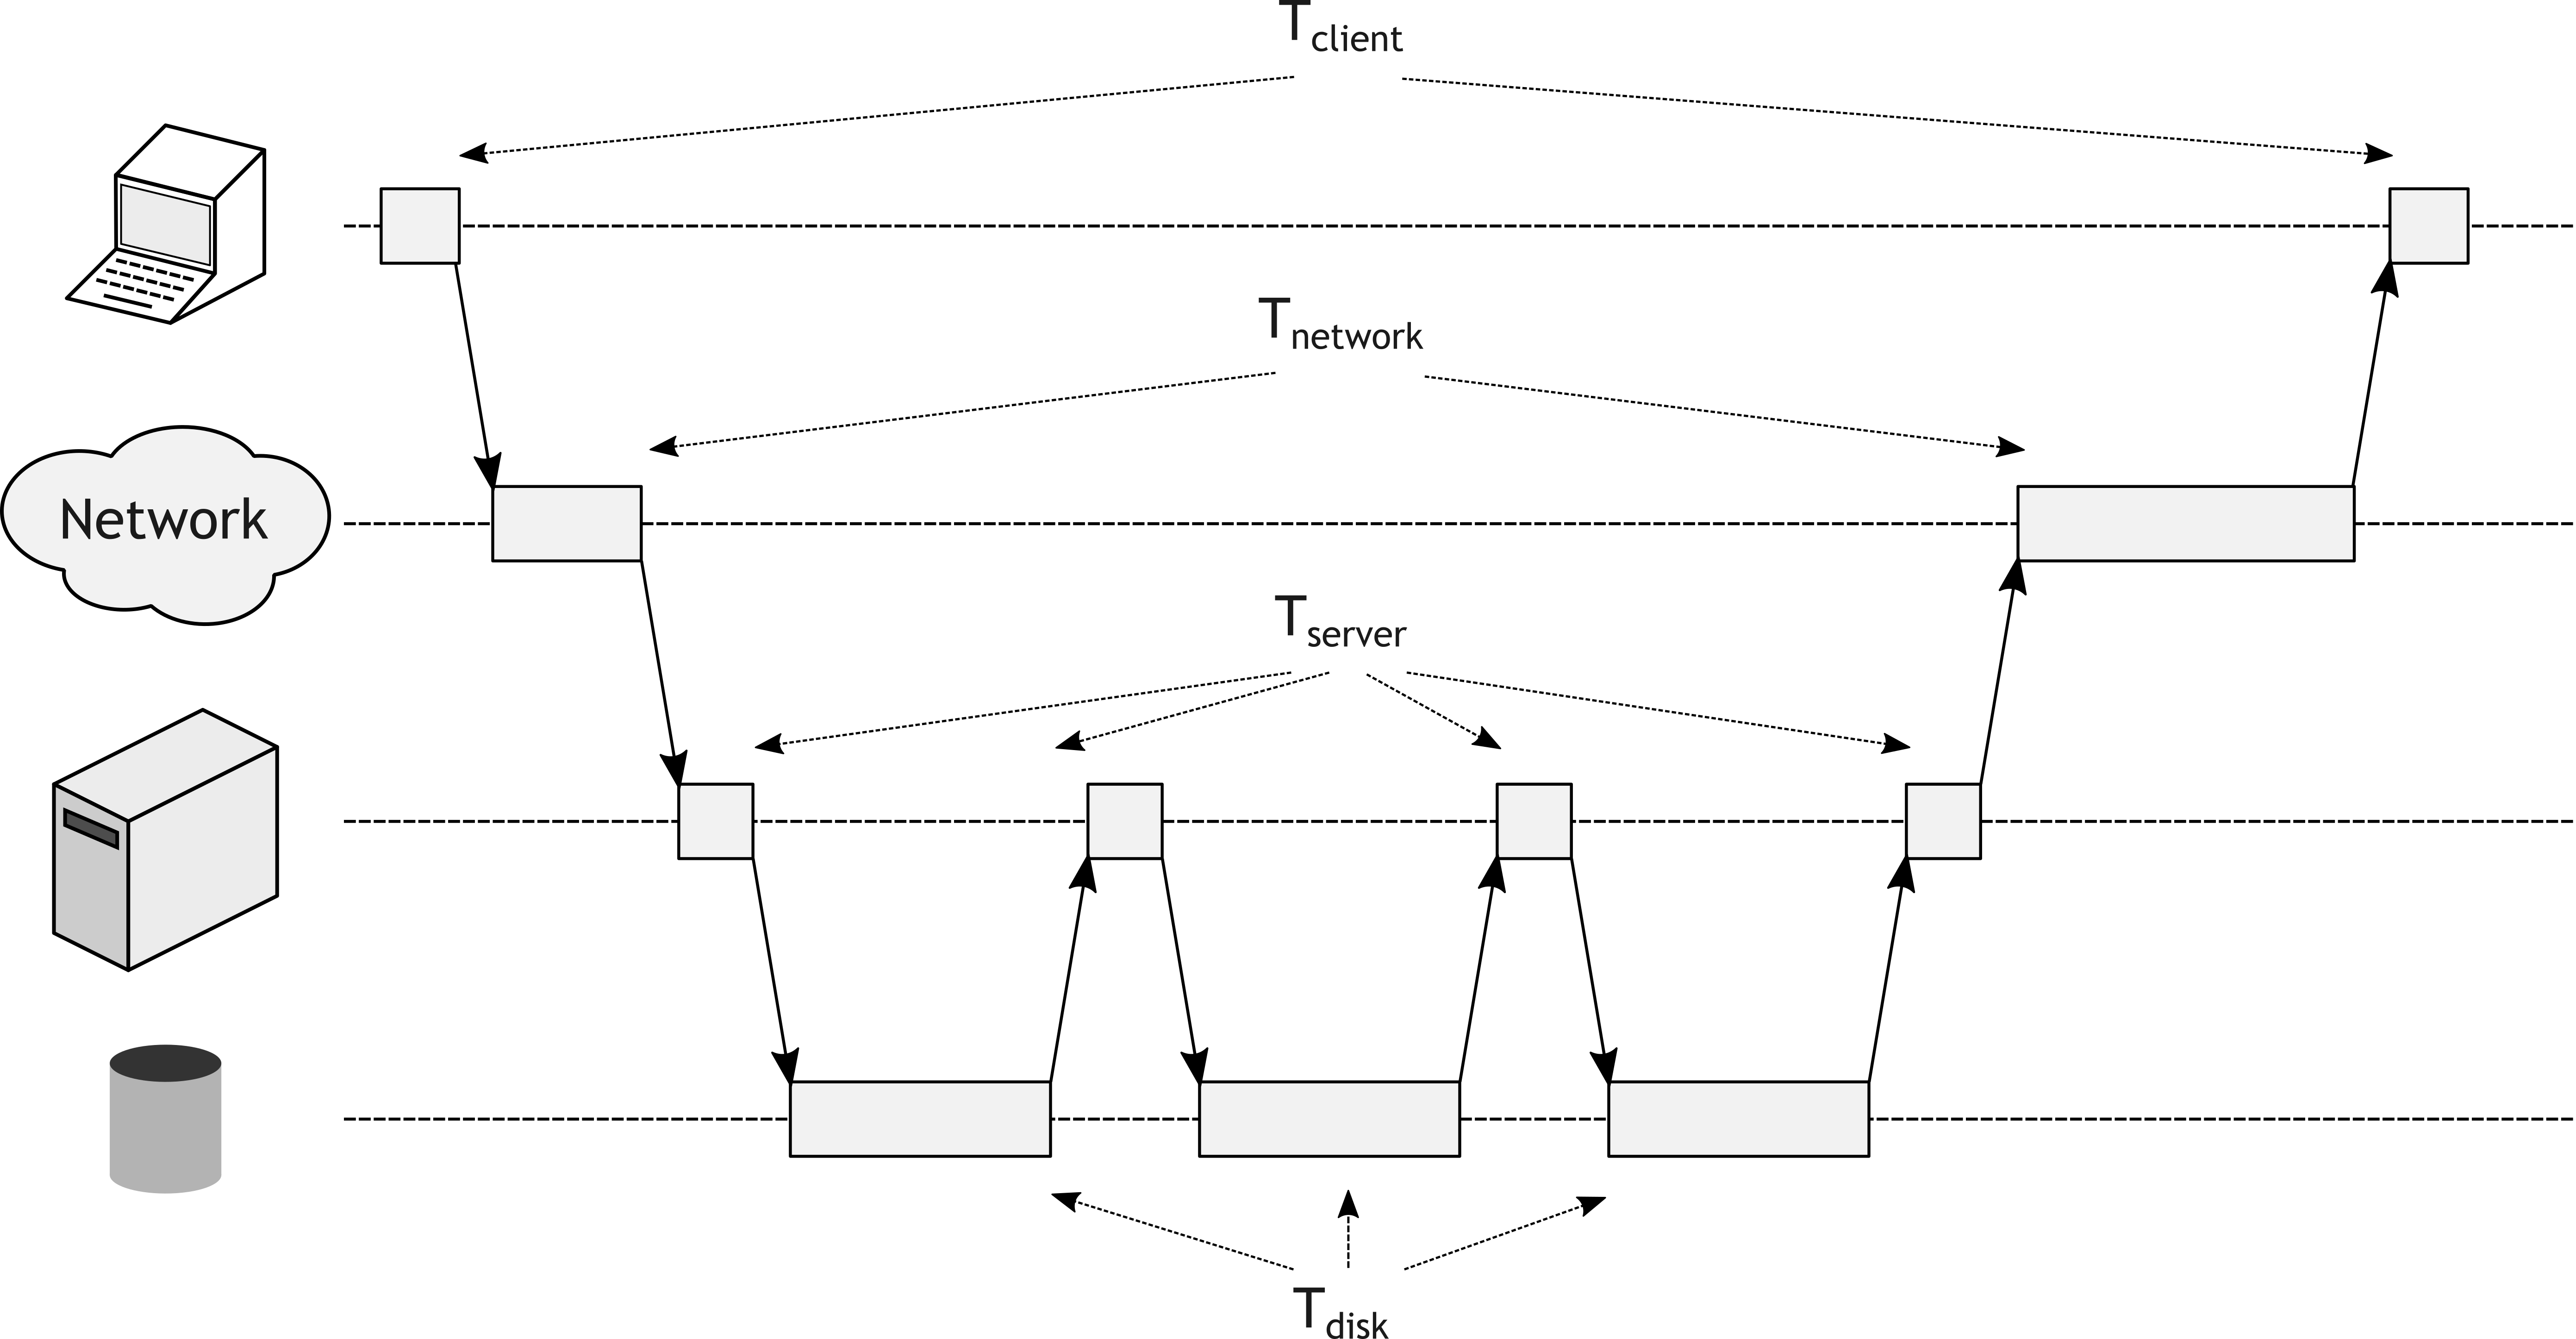
\includegraphics[width=\textwidth]{figures/rpc-request}
\caption{Contribution to I/O time in a distributed storage system.}
\label{figure: rpc-request}
\end{figure}

The time required to perform an I/O operation is given by Equation~\ref{formula: io-time}.
\begin{equation}\label{formula: io-time}
    T_{IO} = T_{client} + T_{network} + T_{server} + T_{disk}
\end{equation}
In this equation there are four contributions, one for each hardware component involved in I/O. $T_{client}$ indicates the time needed by the file system client to initiate and finalize the operation; $T_{network}$ 
indicates the time required to transfer the RPC from the client to the server, and the data from the server back to the client; $T_{server}$ indicates the time between the receiving of the RPC by the server and its 
serving; finally, $T_{disk}$ indicates the time needed to transfer the data from the disk to the server's memory.

In the considered example, a single read operation is converted into multiple server operations because we have assumed data to be laid out in the disk non-contiguously. Normally, file systems try to avoid this 
eventuality but this is not always possible due to file fragmentation. I/O performance is measured in terms of bandwidth by dividing the size of accessed data by the transfer time, as reported in Equation~\ref{formula: io-bw}.
\begin{equation}\label{formula: io-bw}
    BW = \frac{S}{T_{IO}}
\end{equation}

It is important to notice that I/O performance is highly dependent from the way data in the file is accessed. Ideally, we would like to access large chunks of contiguous data through a few requests, which translate 
into a minimum number of network and disk operations. Contrarily, a large number of small non-contiguous requests produces a higher number of network and disk operations. Because scientific codes often access data using
many small non-contiguous requests, additional software layers are used to adapt the application I/O behaviour to the characteristics of the underlying storage system, allowing for better performance. These components
are called middlewares and are positioned between the application and the parallel file system. Middlewares are reviewed in Section~\ref{section: middlewares}.

\subsection{Parallel File Systems}
In Linux systems, and more generally in any UNIX-like system, data is organized into files arranged in a directory tree, or namespace. In Linux everything is represented as a file, including physical I/O 
devices (keyboards, disks, printers, etc), sockets (active network connections), and even operating system statistics (through the \textit{/proc} file system~\footnote{http://man7.org/linux/man-pages/man5/proc.5.html}). 
Files in Linux are accessed through an interface based on the POSIX-IO standard. The standard defines operations to write and retrieve file data as well as metadata. Metadata operations are used to inspect and modify 
file attributes like access permission, creation time, size, and so on. These operations access the file's \textit{inode} (i.e., the file system data structure representing the physical file) along with its attributes. 
Data operations allow users to store and retrieve raw data to and from the file; such data is contained into \textit{data blocks}. Both inodes and data blocks are represented as contiguous byte ranges of size multiple 
of the disk sector, simply called blocks. The block is also the elementary transfer unit in the file system\footnote{The typical sector size in a hard disk is 512~Bytes, while the most common block size is 4~KB (or 8 
sectors).}. Data blocks belonging to the same file are referenced by its inode. Directories are special type of files that do not contain raw data but only key-value pairs. In each of these pairs the key is the name of 
a file inside the directory, while the value is the inode number of the file in the file system. Figure~\ref{figure: inode} shows the relationship between inodes and data blocks in a Linux file system.

\begin{figure}[!htb]
\centering
\includegraphics[width=0.8\textwidth]{figures/inode}
\caption{Simple namespace example and corresponding representation using inodes and data blocks in the file system.}
\label{figure: inode}
\end{figure}

As said, inodes have two sections, one containing file metadata or attributes, and one containing references to data blocks storing raw data. Because inodes and data blocks are of the same fixed size, commonly 4~KB, there 
is a limitation to the number of data blocks that can be directly referenced by an inode, and thus a limit to the file size. If we disregard the attributes and consider 4 bytes addresses, we have that a file cannot be 
bigger than 4~MB (1024 $\times$ 4~KB). For this reason inodes also reference data blocks indirectly through other blocks, the latter storing addresses instead of data. With a single level of indirection, for example, we 
can have an additional 4~GB (1024 $\times$ 1024 $\times$ 4~KB) of space, 4~TB with a double level of indirection.

Parallel file systems~\cite{Braam02}~\cite{SchmuckH02}~\cite{Welch2008}~\cite{CarnsLRT}~\cite{Mcpeek2002} differ from local file systems since instead of storing data into a single hard disk, they use several disks 
connected to remote servers. In most parallel file system designs data is partitioned and spread across many \textit{I/O servers} (IOS), or \textit{data servers} (DS), while metadata, including file mapping information, 
is stored in one or more \textit{metadata servers} (MDSs). The division between data and metadata allows for a specialization of the two services and a better efficiency of the system. The reason is that data and metadata 
access patterns have different characteristics, which can be better addressed by dedicated hardware and software solutions. For example, MDSs are designed to perform a large number of small metadata queries and updates. 
Therefore, besides hard disks, some times they also contain solid state drives that provide better performance for small random accesses; additionally, they are also equipped with larger DRAM memories and more CPU cores. 
I/O servers, on the other hand, are designed for sustaining high aggregated bandwidth for bulk I/O operations and thus have less demanding CPU requirements. Figure~\ref{figure: pfs} shows the high-level architecture of a 
parallel file system.

\begin{figure}[!htb]
\centering
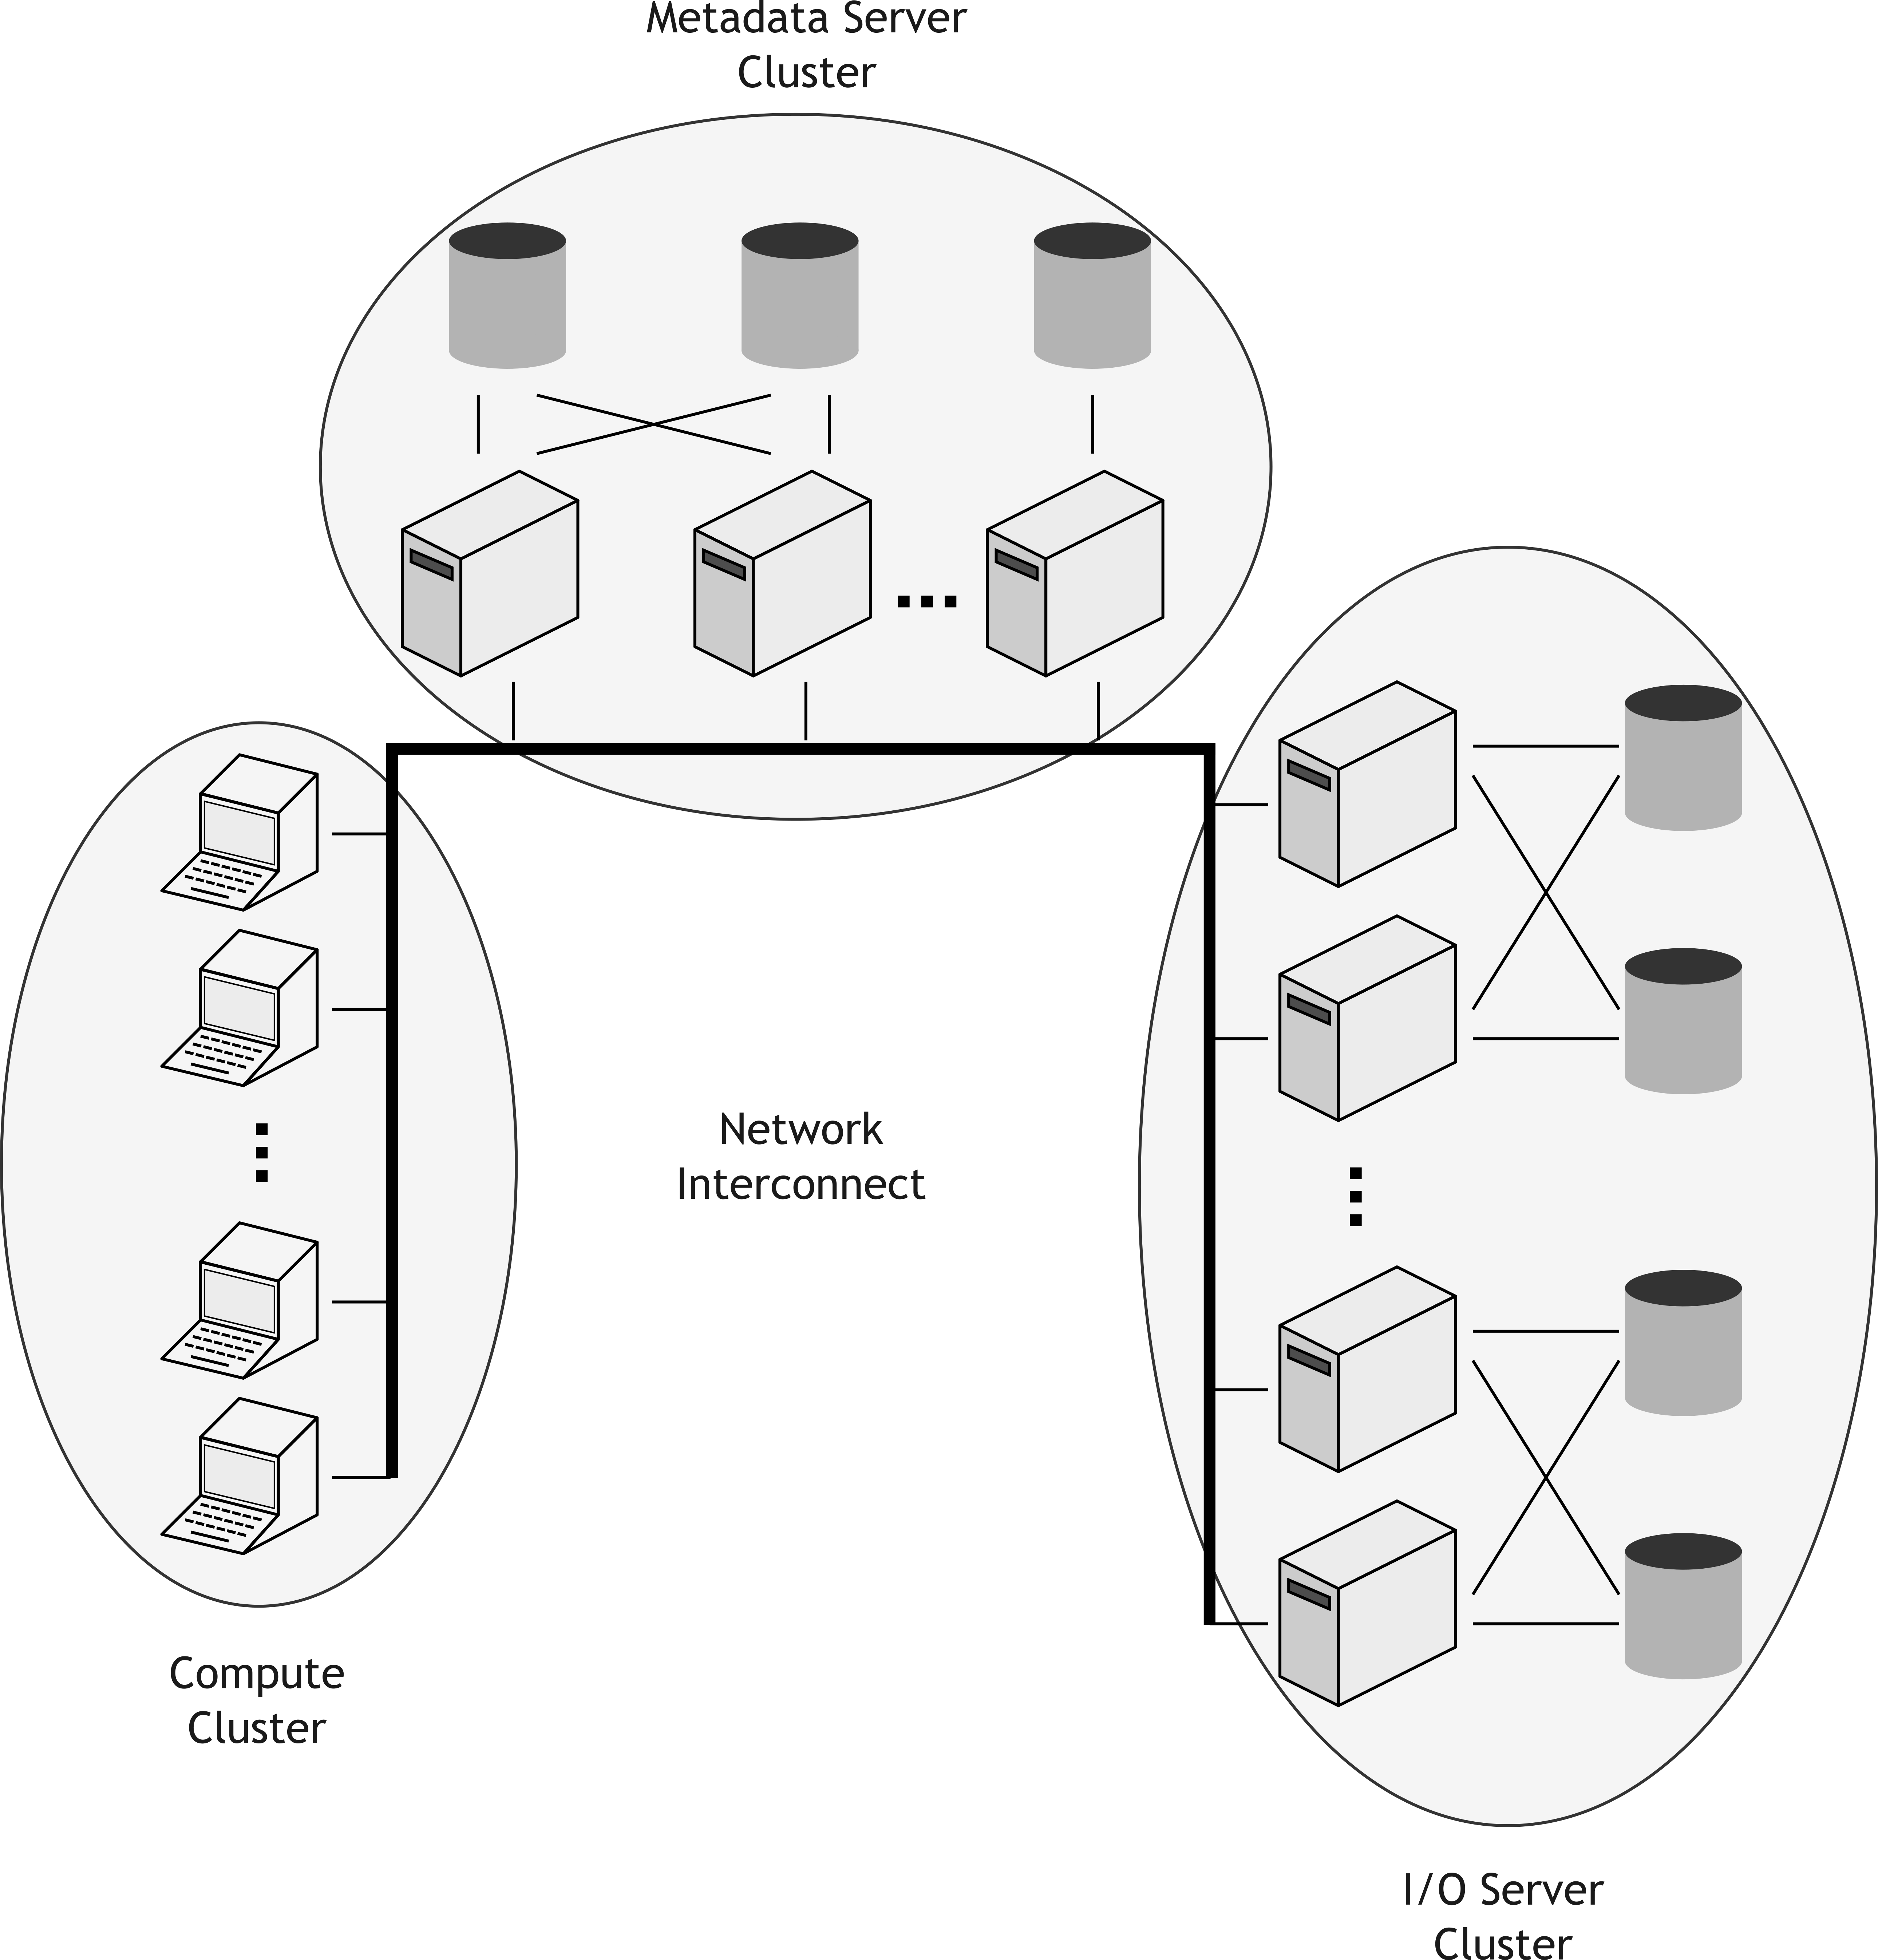
\includegraphics[width=0.8\textwidth]{figures/pfs}
\caption{High-level architecture of a parallel file system.}
\label{figure: pfs}
\end{figure}

Many parallel file systems ultimately rely on local file system installations in the different servers to work. For this reason a distributed file comprises several local files in metadata and data servers. A file, or 
metadata object, in the metadata server is equivalent to an inode in a local file system. It stores all the classical file attributes, plus additional mapping information. Such information allows to determine the location 
of data blocks into IOSs. Mapping attributes are normally represented by three parameters; the first identifies the data server from which the file starts; the second the number of data servers used to store the file, 
also called \textit{striping factor} or \textit{stripe count}; the third the file system block size or \textit{stripe size}. 

In order to uniquely locate blocks in the storage system one additional parameter is needed. This identifies the strategy used to distribute data blocks among the available servers. The simplest and most common strategy 
used is the round robin distribution. I/O servers store data blocks using files, or data objects; for each distributed file, every I/O server has one data object containing a certain number of data blocks, either zero or 
greater than zero.

As said, parallel file systems can use several metadata servers. This allows for better scalability of the metadata service, since the workload can be distributed among several machines. Nevertheless, the file system can 
still suffer poor metadata performance if many processes access the same directory or file at the same time. This is a very common problem in HPC applications that sometime need to create a large number of files in the same
directory, as we will see later. Although metadata distribution can be useful to sustain performance at scale, it also complicates the file system design and creates new problems. One of such problems comes from the fact that 
distributed metadata updates, involving several servers, become possible. Consider Figure~\ref{figure: namespace} as an example. The \texttt{RENAME} of $dir_1/dir_2/dir_4$ to $dir_1/dir_3/dir_4$ involves four servers: $MDS_1$, 
$MDS_2$, $MDS_3$ and $MDS_4$. Indeed, we need to remove the metadata object for $dir_4$ from $MDS_2$ and add it to $MDS_4$. Similarly, we need to remove $dir_4$'s reference from $dir_2$ and add it to $dir_3$.

\begin{figure}[!htb]
\centering
\includegraphics[width=0.8\textwidth]{figures/namespace}
\caption{Example of namespace distributed across four metadata servers.}
\label{figure: namespace}
\end{figure}

If distributed metadata updates are not handled properly, a server crash may lead to inconsistencies. To avoid this eventuality file systems employ appropriate distributed commitment protocols. The drawback this time 
is that these protocols involve the exchange of a large number of network messages and synchronous writes to disk in order to safely commit a metadata update~\cite{Stamos1990}~\cite{Gray2006}, thus impacting performance. 
Distributed metadata services in parallel file systems have been widely studied~\cite{Zhang2001}~\cite{Fan2004}~\cite{Michalak2005}~\cite{Sinnamohideen2010}~\cite{Congiu2012}, but there is no best solution that can fit 
every use case.

\subsubsection{Consistency Semantics}
All information processing systems are composed by a set of hardware and software components that communicate with each other through electric signals and messages. The simplest computer, for example, is composed by at 
least one CPU, some amount of DRAM memory, one hard disk and the operating system. The CPU executes programs' instructions, loads data from the disk into the DRAM, modifies data in the DRAM and possibly writes it 
back to the disk. Assuming that the executed program is coded properly and does not contain any bug, we want to make sure that its execution in the computer always generates the same result and that this result is the 
correct one.

We focus our attention on the disk subsystem and more specifically on the file system software responsible for storing and retrieving data. In this case we want to make sure that the subset of operations involving I/O 
does not alter the correct program execution; that is, if the program completes it generates the right result. In the case of the file system, and generally of every other software component, this boils down to 
the identification of a set of invariants and the enforcement of the condition that these are respected before and after every I/O operation. These conditions translate into a list of semantic requirements for the
file system's operations. 

A very common semantic model, especially in relational databases, is the ACID model~\cite{Gray1981}~\cite{Wright2007}. ACID stands for \textit{atomicity}, \textit{consistency}, \textit{isolation} and \textit{durability}. 
Atomicity means that if a file system operation is composed by multiple steps, either all of them complete or neither of them completes; consistency means that every operation takes the file system from one valid 
state to another; isolation means that the concurrent execution of multiple file system operations is equivalent to their sequential execution and; finally, durability means that once an operation has completed its 
effects cannot be lost, even in the presence of a system crash.

The POSIX-IO standard only enforces atomicity and consistency. Durability is not considered because it would result in serious performance penalties. For example, in a durable file system every write operation should be
carried out synchronously. Because disks are orders of magnitude slower than CPUs, the program would spend most of its time waiting on I/O, thus making little progresses. To avoid this, data and metadata updates are 
applied to DRAM and are committed to disk only explicitly by the user through the invocation of either \texttt{sync()} or \texttt{close()} of the file. Isolation is also not considered because it would require the file 
system to lock every data structure that can be accessed concurrently, even if this does not violate any invariant. However, the lack of isolation leaves programs open to vulnerabilities due to race conditions. For example, 
if the execution of an operation in one program depends on the value of a certain variable that can be modified by another process after it was read, the program might perform an operation that relies on a condition that 
is no longer true. This is known as \textit{Time-of-check-time-of-use} (TOCTOU)~\cite{Wright2007} problem.

In a distributed system, like a parallel file system, atomicity and consistency requirements are particularly hard to enforce and require the implementation of special distributed locking mechanisms. Consistency, for
example, requires that every write operation becomes immediately visible to every node accessing the file. This is equivalent to saying that all the caches in the different nodes have to be coherent with the data in the 
file. One problem in this sense comes from the so called \textit{false sharing} of file system blocks. Because file systems write data at the block granularity, if two nodes write to the same block, even though the writes 
do not overlap, the last writer will end up overwriting the other node's data, causing data inconsistencies and wrong results. This condition is shown in Figure~\ref{figure: false-sharing} and is normally solved by 
implementing locks at the block granularity. False sharing also causes performance degradation because it forces the file system to perform read-modify-write to partially update a block. Lock contention and extra read 
overhead are important aspects that users have to keep in mind when reaching out for high performance data access in their codes.

\begin{figure}[!htb]
\centering
\includegraphics[width=0.9\textwidth]{figures/false-sharing}
\caption{In this case false sharing of block two in the file can lead to two different outcomes. In the first case process $P_1$ writes before $P_0$, in the second case the order is inverted.}
\label{figure: false-sharing}
\end{figure}

The locking strategy is implemented differently by different file systems. Nevertheless, in order to reduce overhead and improve performance, most solutions use an extent based locking~\cite{Braam02}~\cite{SchmuckH02}. In the 
extent based locking the file system client requesting exclusive access to a file region, is granted a lock for a larger extent, multiple of the block size. Because programs do not access only one part of the file, the extent 
based approach allows them to avoid acquiring further locks from the lock manager for future accesses.

Atomicity is frequently enforced through the \textit{write ahead logging} (WAL) of file system metadata, also called journaling. In WAL metadata updates are not committed to the disk immediately but are instead logged into a 
journal. Every once in a while, or when the user explicitly requests it (e.g., through \texttt{sync()}), data is written to the file and afterwards the journal is forced to disk as well. For example, if the user creates a 
new file, the journal will contain two entries, one for the allocation of the new inode and one to add a reference to the inode in the parent directory (link). Upon a system crash and restart the file system inspects the 
log to check whether the create operation has completed successfully (all the relevant data structures have been updated) or has completed only partially. If the operation has completed the corresponding entries can be removed 
from the journal, while if the operation has completed partially the file system can decide whether to complete it or undo the partial changes. (In any case the file system is always recovered to a consistent state. While WAL 
is used in many file systems, other solutions are also possible like, for example, \textit{copy-on-write}.) The advantage of using journaling is that in the eventuality of a crash, upon restart, the file system does not need 
to scan the all disk to verify if any of its data structures has been left into an inconsistent state, which is a time consuming operation that in large disks can require up to several hours.

\subsection{I/O Gap}
Moore's law has been driving technological advancements in integrated circuits for the past five decades, almost doubling density and speed of microprocessor every two years~\cite{Mack11}. Comparable technological advancements 
in hard disk drives (HDDs) have been achieved for capacity increase~\cite{Grochowski1996}~\cite{NIST} but not for latency reduction. As shown in Figure~\ref{figure: hdd-trend}, areal density has been increasing steadily at a 
rate of 100\% every year since 1997. This trend slowed down to 30\% in 2001 to start growing again at 50\% in 2005. Today, the areal density increase is 40\% per year~\cite{Masakatsu2015}. Unlike density, latency improvements 
are limited by the speed at which mechanical parts in the disk can move. Several research works have tried to alleviate the impact of mechanical latency on performance by proposing more efficient strategies to schedule disk 
requests~\cite{jacobson1991}~\cite{Worthington1994}~\cite{Iyer2001}.

\begin{figure}[!htb]
\centering
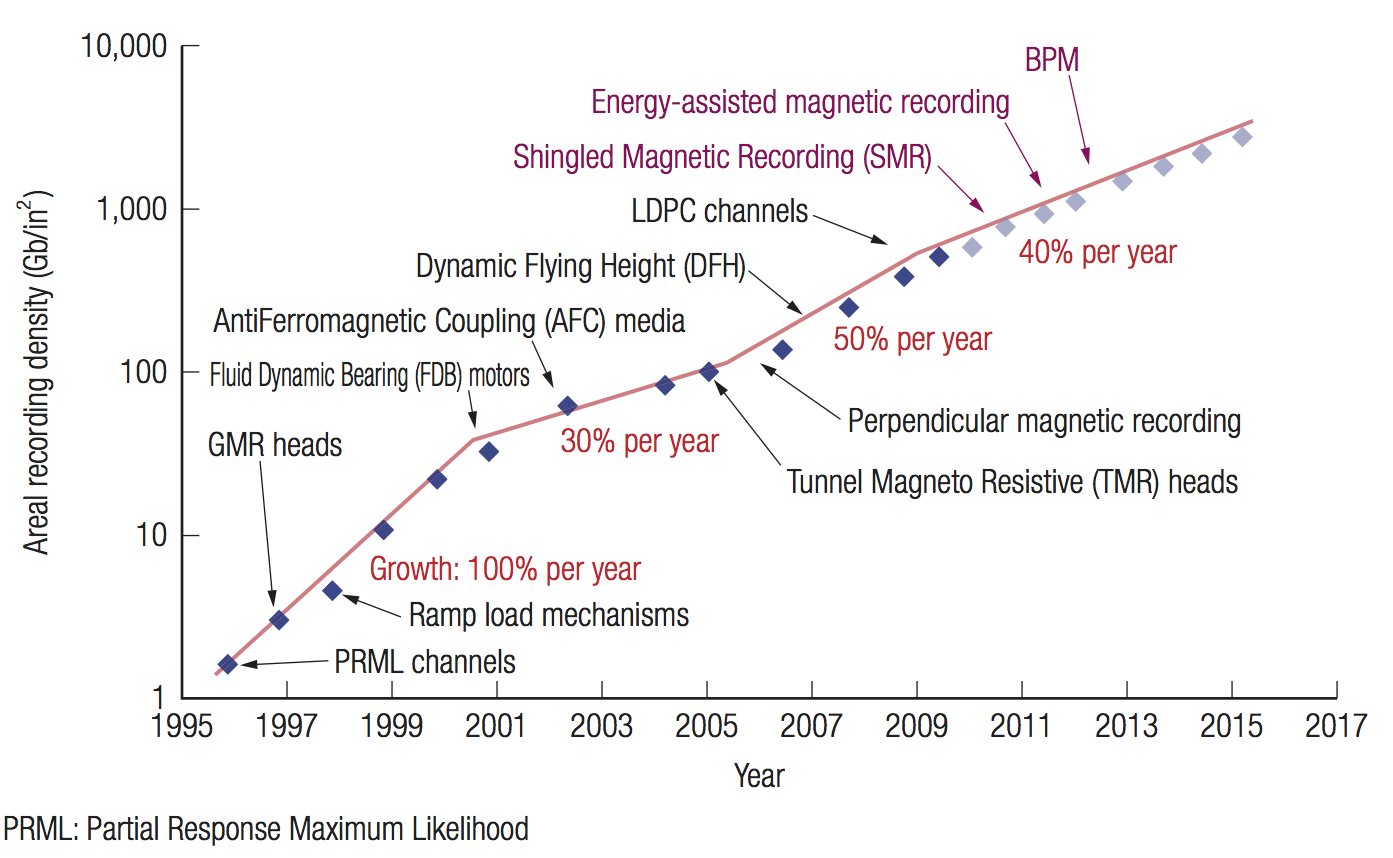
\includegraphics[width=0.8\textwidth]{figures/hdd-trend}
\caption{Recording density has been improved thanks to technological advancements in different fields including magnetic sensors and recording mediai~\cite{Shiroishi2009}.}
\label{figure: hdd-trend}
\end{figure}

The technological gap between CPUs and hard disks, also known as \textit{I/O gap}, has caused performance of HDDs to fall far behind compute components, imposing time penalties of millions of CPU cycles on 
applications performing I/O operations. This problem is particularly relevant in HPC environment because the performance of compute components increases much faster than storage, as shown in Table~\ref{table: hpc-trend}
~\cite{ASCAC2010}. The table compares the characteristics of a typical 2010 supercomputer with the characteristics of future Exascale machines, which were predicted to be available in 2018. Exascale machines are not yet 
available and will not be available by the 2018 time frame. More recently, the U.S. \textit{departmment of energy} (DOE) \textit{advanced scientific computing research} (ASCR) initiative has worked on updating the requirements 
of HPC systems at Exascale for different areas of interest including \textit{high energy physics} (HEP)~\cite{HEP2015}, \textit{basic energy sciences} (BES)~\cite{BES2015}, \textit{fusion energy sciences} (FES)~\cite{FES2016}, 
\textit{biological and environmental research} (BER)~\cite{BER2016} and \textit{nuclear physics} (NP)~\cite{NP2016} through the 2025 time frame. What has emerged from the updated requirement reviews is that initial estimates of
hardware resources, as presented in the first ASCAC report~\cite{ASCAC2010}, are a coarse grain approximation coming from a static projection of 2010 systems to 2018. As an example, the pre-exascale 180 PFlops Aurora system that 
will be installed at the \textit{Argonne leadership computing facility} (ALCF) in 2018 is expected to have an I/O bandwidth of only 1~TB/s. This bandwidth is aligned with currently installed systems, like the Cray Blue Water 
supercomputer. For this reason, although the projections in Table~\ref{table: hpc-trend} are seven years old, here we assume they provide an upper bound coarse grain approximation that is valid for the development of this
dissertation.

\begin{table}[!htb]
    \centering
    \ra{1.5}
    \caption{Potential Exascale Computer Design for 2018 and its relationship to current HPC designs.}
    \newcolumntype{A}{>{\arraybackslash} m{4cm}}
    \newcolumntype{B}{>{\centering\arraybackslash} m{2cm}}
    \newcolumntype{C}{>{\centering\arraybackslash} m{2cm}}
    \newcolumntype{D}{>{\centering\arraybackslash} m{2cm}}
    \begin{tabular}{ABCD}
        \toprule
        & \bf \small 2010 & \bf \small 2018 & \bf \small Factor Change \\
        \midrule
        \small System Peak         & \small 2 Pf/s     & \small 1 Ef/s     & \small 500   \\
        \small Power               & \small 6 MW       & \small 20 MW      & \small 3     \\
        \small System Memory       & \small 0.3 PB     & \small 10 PB      & \small 33    \\
        \small Node Performance    & \small 0.125 Gf/s & \small 10 Tf/s    & \small 80    \\
        \small Node Memory BW      & \small 25 GB/s    & \small 400 GB/s   & \small 16    \\
        \small Node Concurrency    & \small 12 cpus    & \small 1,000 cpus & \small 83    \\
        \small Interconnect BW     & \small 1.5 GB/s   & \small 50 GB/s    & \small 33    \\
        \small System Size (nodes) & \small 20 K nodes & \small 1 M nodes  & \small 50    \\
        \small Total Concurrency   & \small 225 K      & \small 1 B        & \small 4,444 \\
        \small Storage             & \small 15 PB      & \small 300 PB     & \small 20    \\
        \small I/O Bandwidth       & \small 0.2 TB/s   & \small 20 TB/s    & \small 100   \\
        \bottomrule
    \end{tabular}
    \label{table: hpc-trend}
\end{table}

Table~\ref{table: hpc-trend} estimates that peak performance for Exascale systems will increase by a factor of 500, while I/O bandwidth will only increase by a factor of 100. This will cause a farther widening of the 
I/O gap and lead to serious scalability limitations for large scale simulations. To address this problem scientists are investigating deep memory hierarchies as well as non-volatile byte addressable memory technologies
~\cite{Wang2013}~\cite{Zhang2015}~\cite{Breitwisch2008}. 
Some of these technologies, like flash based \textit{non-volatile memory} (NMV) devices, are already used as storage accelerators in so called \textit{burst buffers}. We will discuss memory technologies in Section~\ref{section: mem-tech} 
and bust buffers in Section~\ref{section: caching}.

\subsection{Small I/O}
HPC applications often exhibit irregular I/O patterns that are not handled efficiently by the parallel file systems. Indeed, most scientific codes comply to the \textit{single program multiple data} (SPMD) model 
in the Flynn taxonomy. This means that a single program is executed concurrently by an ensemble of nodes in the cluster; each instance performs the same set of operations but on a different portion of a larger 
multi-dimensional domain. Because data is organized as sequence of blocks on disk, parallel I/O from the application to the different portions of the dataset might translate into a large number of, possibly small, 
non-contiguous requests that are notoriously serviced inefficiently by hard disk drives~\cite{Nieuwejaar1996}~\cite{Simitci1998}. This problem is also known as the \textit{small I/O problem}, and is typically 
addressed by specific software components called I/O middlewares. 

\begin{figure}[!htb]
\centering
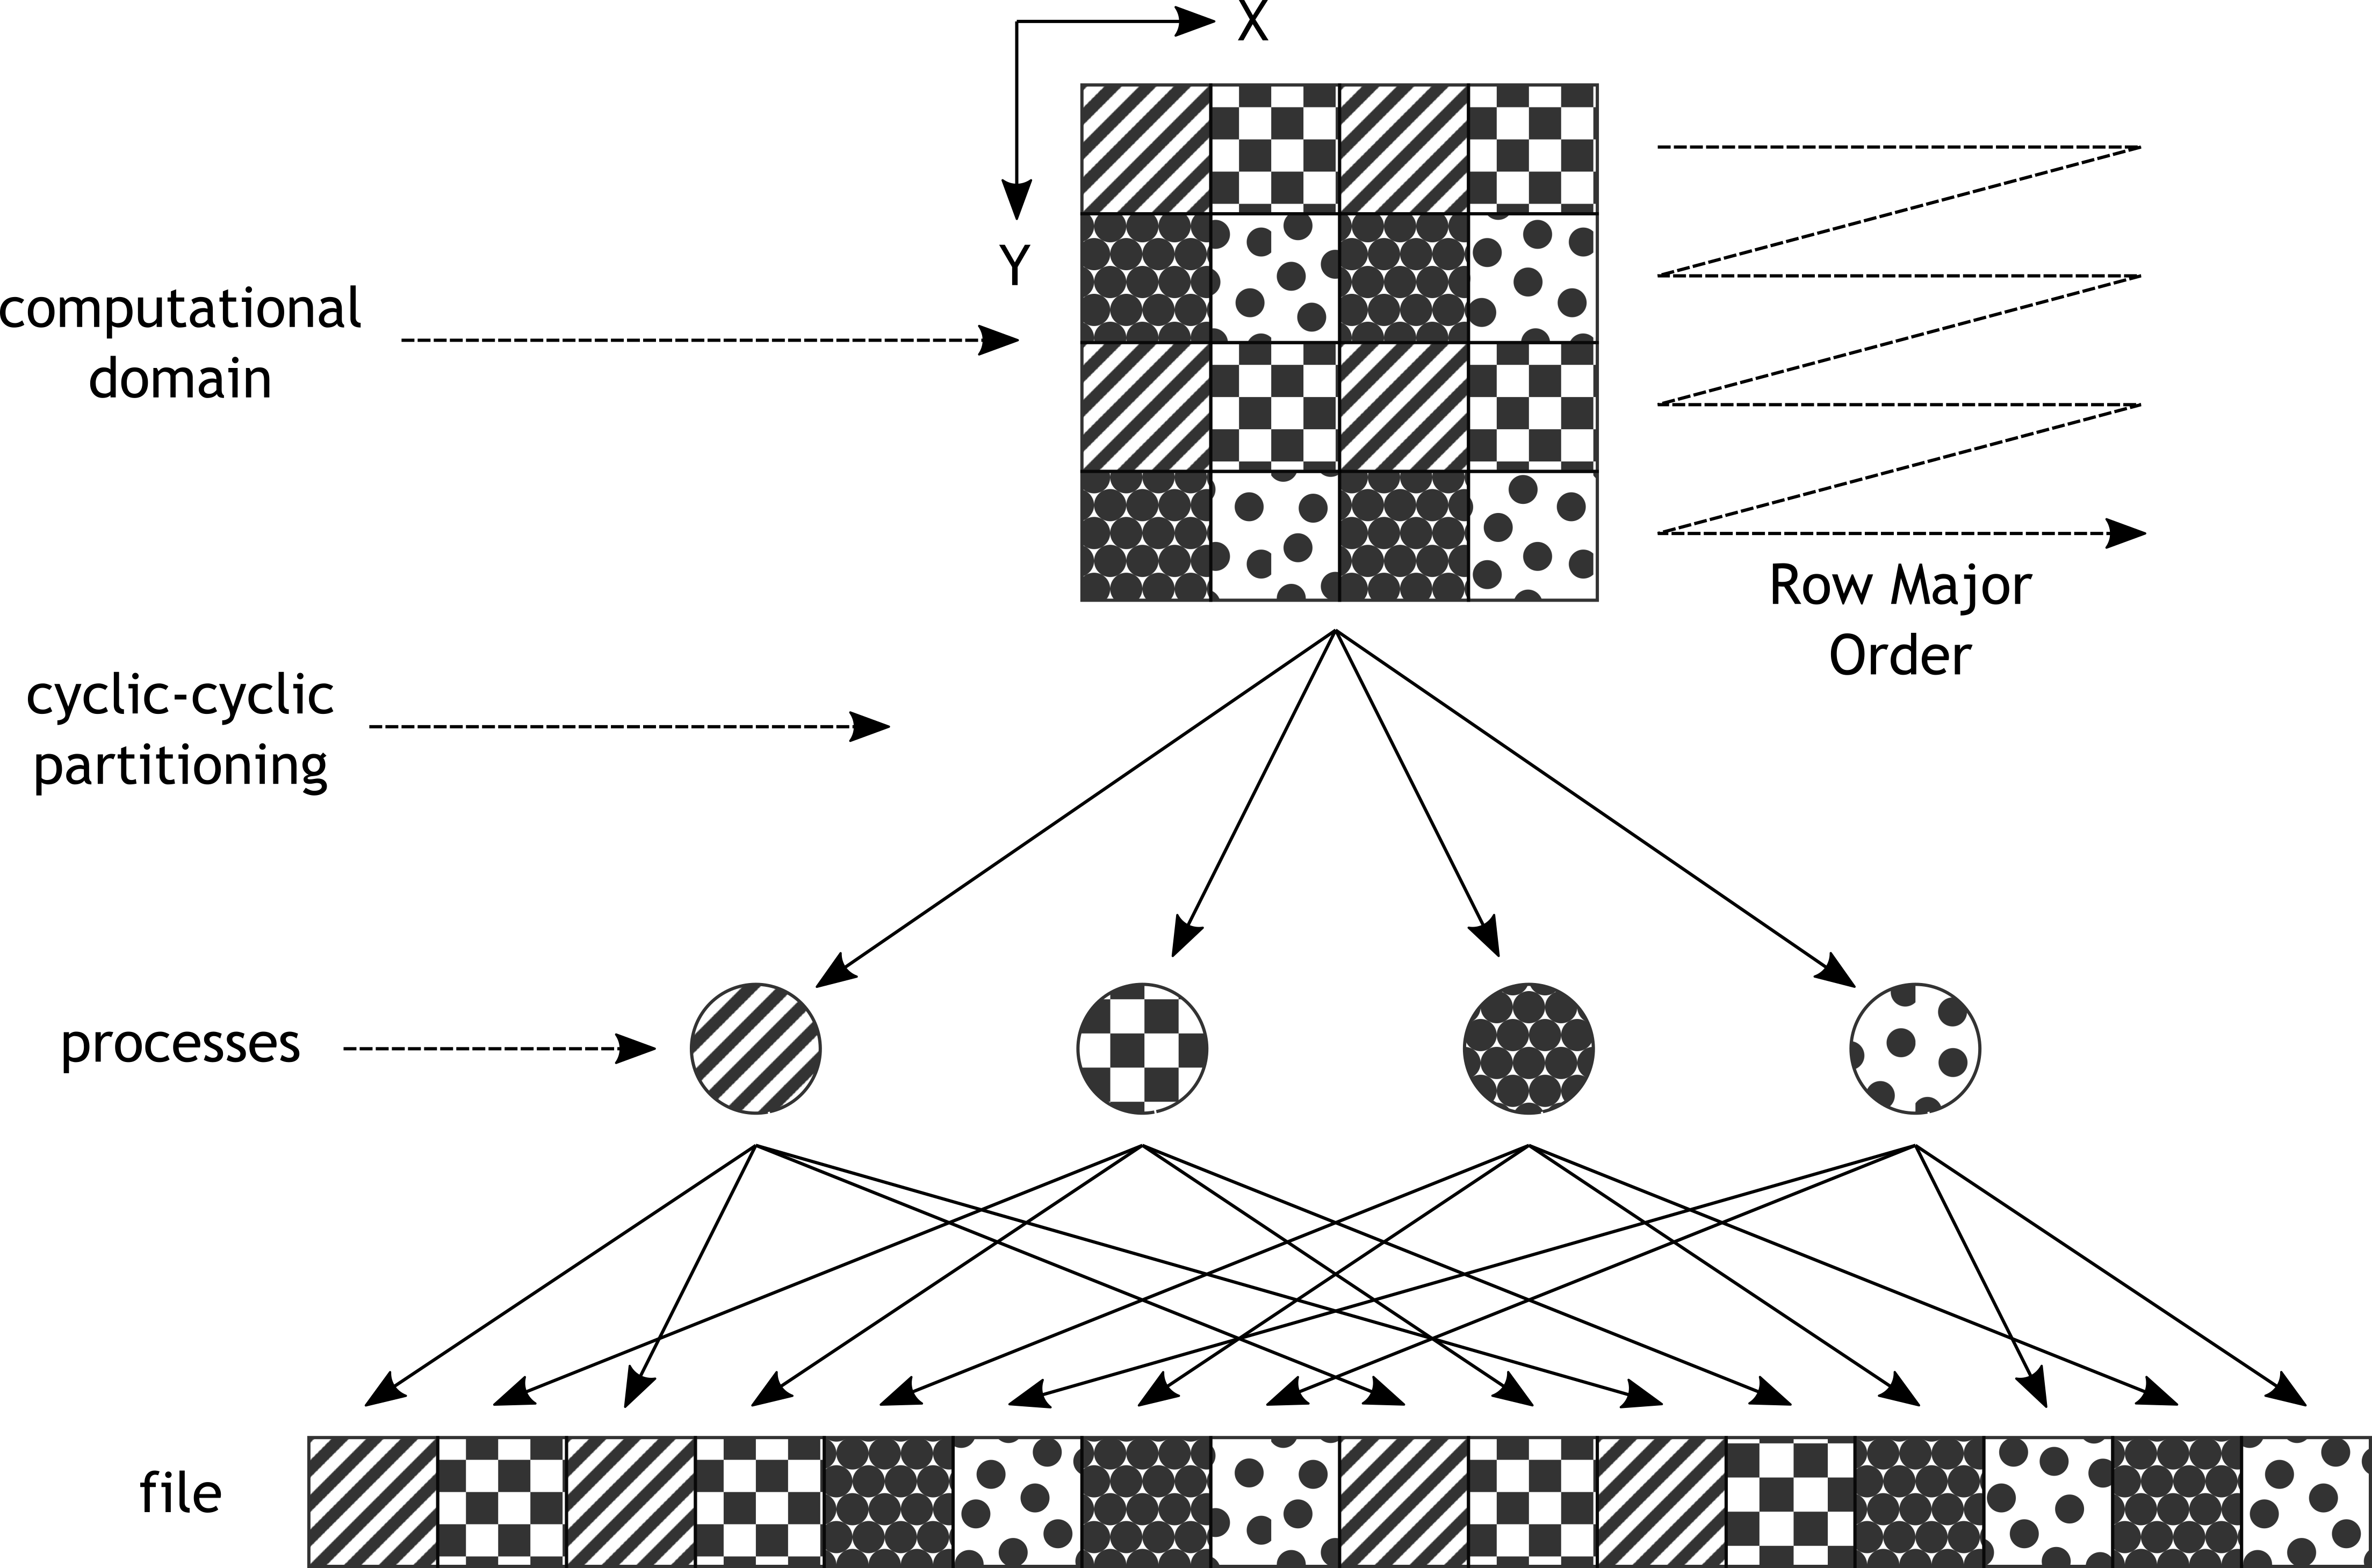
\includegraphics[width=0.8\textwidth]{figures/small-io}
\caption{Example of two-dimensional domain partitioning in parallel applications. The original domain is divided among four processes using a cyclic-cyclic partitioning strategy. Each process in the application 
performs its tasks on the data and then writes the results to a shared file concurrently.}
\label{figure: small-io}
\end{figure}

To better understand why small I/O is a problem consider a simple two-dimensional dataset as show in Figure~\ref{figure: small-io}. In the example, the original domain is divided into smaller sub-domains which are afterwards 
assigned to the available processes for computation using a cyclic-cyclic partitioning strategy~\cite{delRosario1993}; that is, the domain is first divided into four blocks and inside each of these data is assigned to the available processes 
cyclically\footnote{Many other domain partitioning strategies are possible and each of these reflects differently on the access pattern characteristics of the application.}. Every process performs its tasks and then concurrently 
writes the results into a shared file using the row-major order\footnote{The input domain is scanned row by row and mapped onto a single dimensional representation in the file.}.

The row-major mapping of the original domain onto the file destroys the original locality of data and because I/O is performed independently, without any coordination among the processes, the file system cannot guarantee that 
accesses will be served in an ordered way by increasing offset. On the contrary, requests will most likely arrive out of order, generating an increased seek activity in the disks, stalling the application on I/O for a long time. 
Moreover, because the size of the sub-domains can be very small, disks might spend most of the time seeking from one point of the file to the other, underutilizing the available throughput. Another deleterious effect of 
uncoordinated I/O is the false sharing of file system blocks, that results in expensive communication between the application and the file system's lock manager to acquire and release exclusive access rights to the file regions 
of interest. This produces the serialization of I/O operations and further increases the I/O stall time.

As we will see in the rest of the chapter this problem is commonly addressed by reorganizing and consolidating I/O requests generated by file system clients (i.e., application's processes) to match the logical distribution 
of data blocks in the file. In this way a smaller number of large sequential requests is presented to the disks, also minimizing file system block contention and ultimately I/O stalls. Some of the middlewares that we will 
review address this problem by converting parallel I/O to the shared file into parallel I/O to independent files (PLFS~\cite{Bent2009}). Others leverage global access pattern knowledge exposed by processes to make sure that I/O operations 
are intelligently coordinated (e.g., ROMIO~\cite{ThakurC96}, ADIOS~\cite{Lofstead2008}).

\subsection{Checkpointing}
Large scale HPC systems are subject to the failure of hardware components~\cite{Schroeder2006}~\cite{Schroeder2007} and to soft errors~\cite{Michalak2005}. Such failures represent a threat for long time running applications 
that in such cases would need to restart their execution from scratch, loosing all the progresses made and wasting precious time and system resources. For this reason, parallel applications typically divide their execution 
into multiple phases of computation, interleaved by periods of intense write activity during which the execution context is pushed to stable storage, also called checkpoints. In the eventuality of a system failure, the application 
can pick up computation from the most recent checkpoint, thus saving time. 

Clearly checkpointing is a viable technique but since I/O is expensive, applications should make sure they do not abuse it; that is, checkpoints should not be written more often than strictly necessary. Therefore, the checkpointing 
interval should be chosen to minimize the wall-clock execution time of the application. An estimate of the execution time as a function of the checkpoint interval is given by Daly~\cite{Daly2006}. More recent works look at the severity 
of the failures and propose a multi-level checkpointing approach in which parallel file system checkpoints are extended with node local storage checkpoints~\cite{Moody2010}~\cite{Moody2010_2}. This approach exploits local storage for 
less critical failures and relies on the parallel file system only for the most critical failures, that cannot reconstruct the requested checkpoint data from the local storage devices. %in Equation~\ref{formula: jtdaly}.

%\begin{equation}\label{formula: jtdaly}
%    T_w = M e^{\frac{R}{M}} \left( e^{\frac{\tau + \delta}{M}} - 1 \right) \left( \frac{T_I}{\tau} - \frac{\delta}{\tau + \delta}\right)
%\end{equation}

%The wall-clock execution time $T_w$ in Equation~\ref{formula: jtdaly} depends from the checkpoint interval length $\tau$, the system mean time between failures $M$, the time required to create a new checkpoint $\delta$, 
%the time needed to restart the application $R$ and the ideal uninterrupted execution time of the application $T_I$. Additionally, the optimal checkpoint interval length that minimizes \ref{formula: jtdaly} is given by
%\ref{formula: optimal-checkpoint}.

%\begin{equation}\label{formula: optimal-checkpoint}
%    \tilde\tau = \begin{cases}
%        \sqrt{2 \delta M} \left(1 + \frac{1}{3} \sqrt{\frac{\delta}{2 M}} + \frac{1}{9} \frac{\delta}{2 M} \right) - \delta \qquad \text{$\delta < 2 M$}\\
%        M \qquad \qquad \qquad \qquad \qquad \qquad \qquad \quad \text{$\delta \geq 2 M$}
%    \end{cases}
%\end{equation}

%The asymptotic checkpointing efficiency can be computed by $\eta = lim_{T_I \rightarrow \inf} \frac{T_I}{T_w}$. Clearly, in order to have a good efficiency, this limit needs to be as close as possible to 1. For a detailed 
%discussion and derivation of the reported equations please refer to the Daly work.

Due to their sensitivity to system failures, checkpointing has become one of the most predominant I/O patterns in HPC applications. Applications perform checkpointing using two different write strategies. In the first case, 
every process writes its state to a separate file, also called N to N pattern, or N-N for short. In the second case, every process writes its state to a single shared file, also called N to 1 pattern, or N-1 for short. 
Because applications need to guarantee that processes running on different physical nodes in the system progress together in their compute tasks, they use barriers (i.e., global synchronization points in the code) to avoid 
the implementation of expensive distributed synchronization algorithms~\cite{Lamport1978}. Unfortunately, when transferring application state to stable storage, the use of barriers just pushes the synchronization burden 
from the application to the parallel file system, that has to guarantee data consistency implementing mutual exclusion through locking.

\begin{figure}[!htb]
  \centering
  \begin{subfigure}[t]{0.46\textwidth}
  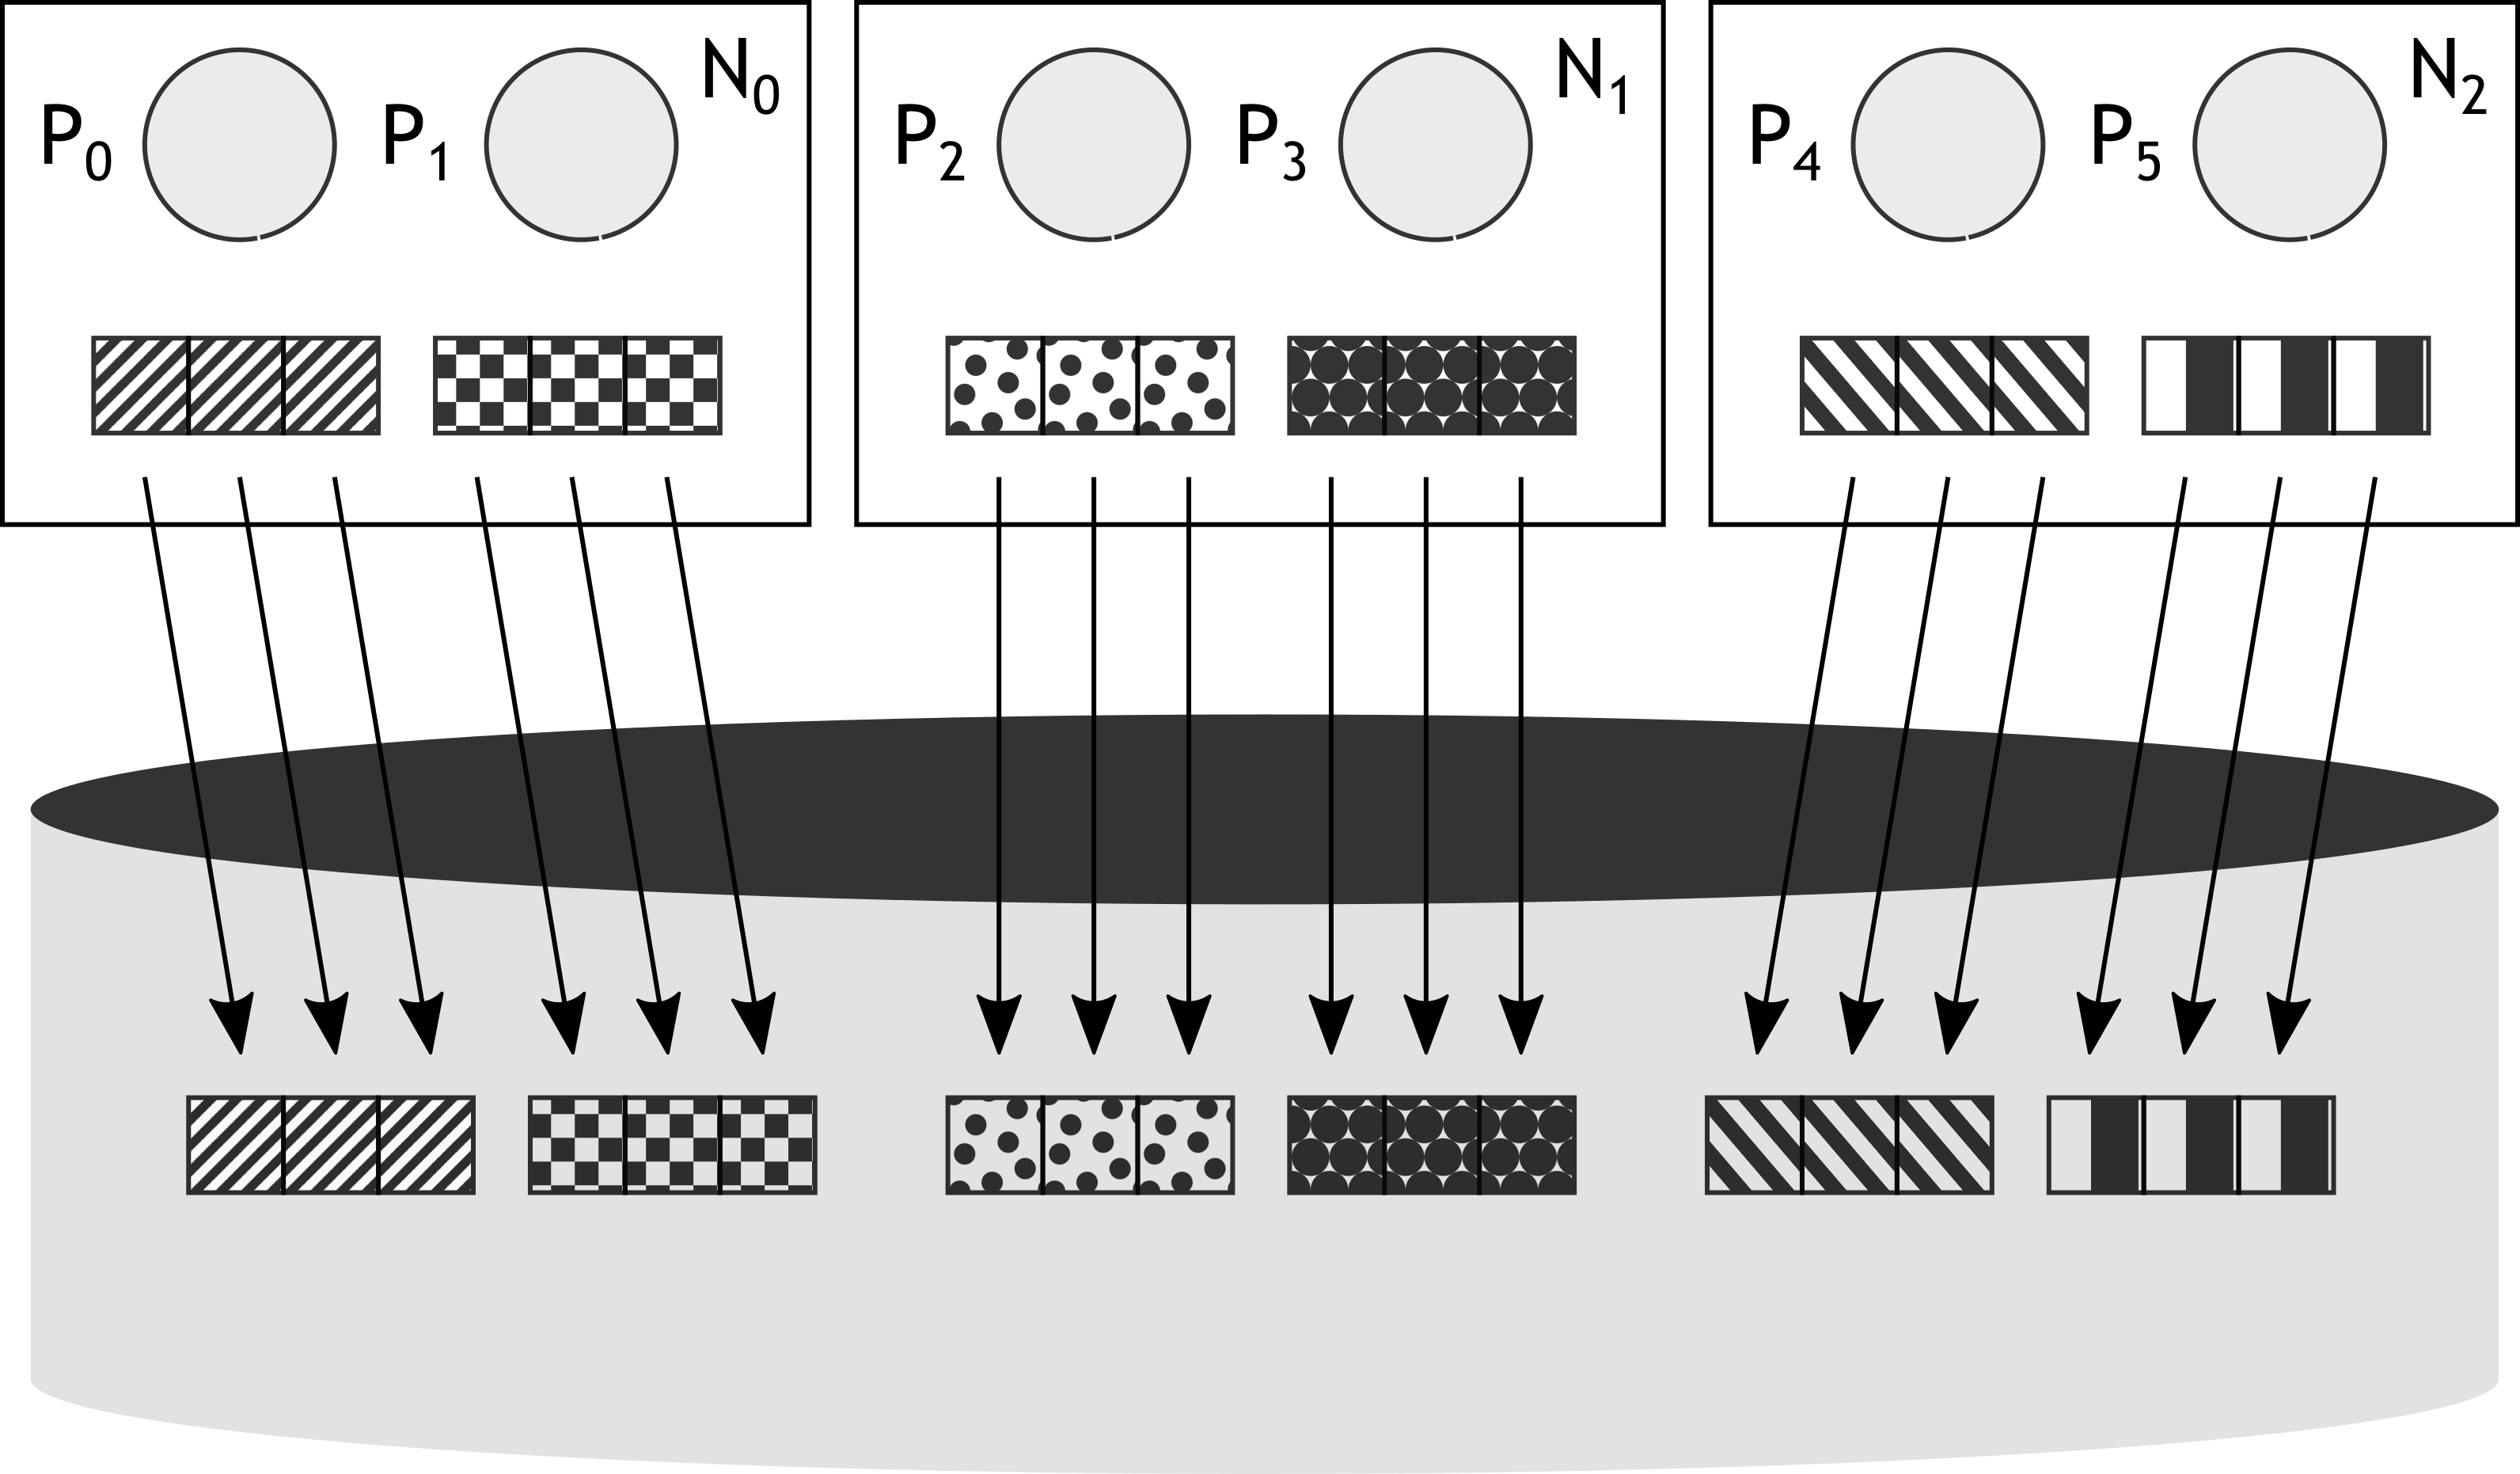
\includegraphics[width=\textwidth]{figures/checkpoint-n-n}
  \caption{N-N pattern.}
  \label{figure: checkpoint-n-n}
  \end{subfigure}
  \begin{subfigure}[t]{0.46\textwidth}
  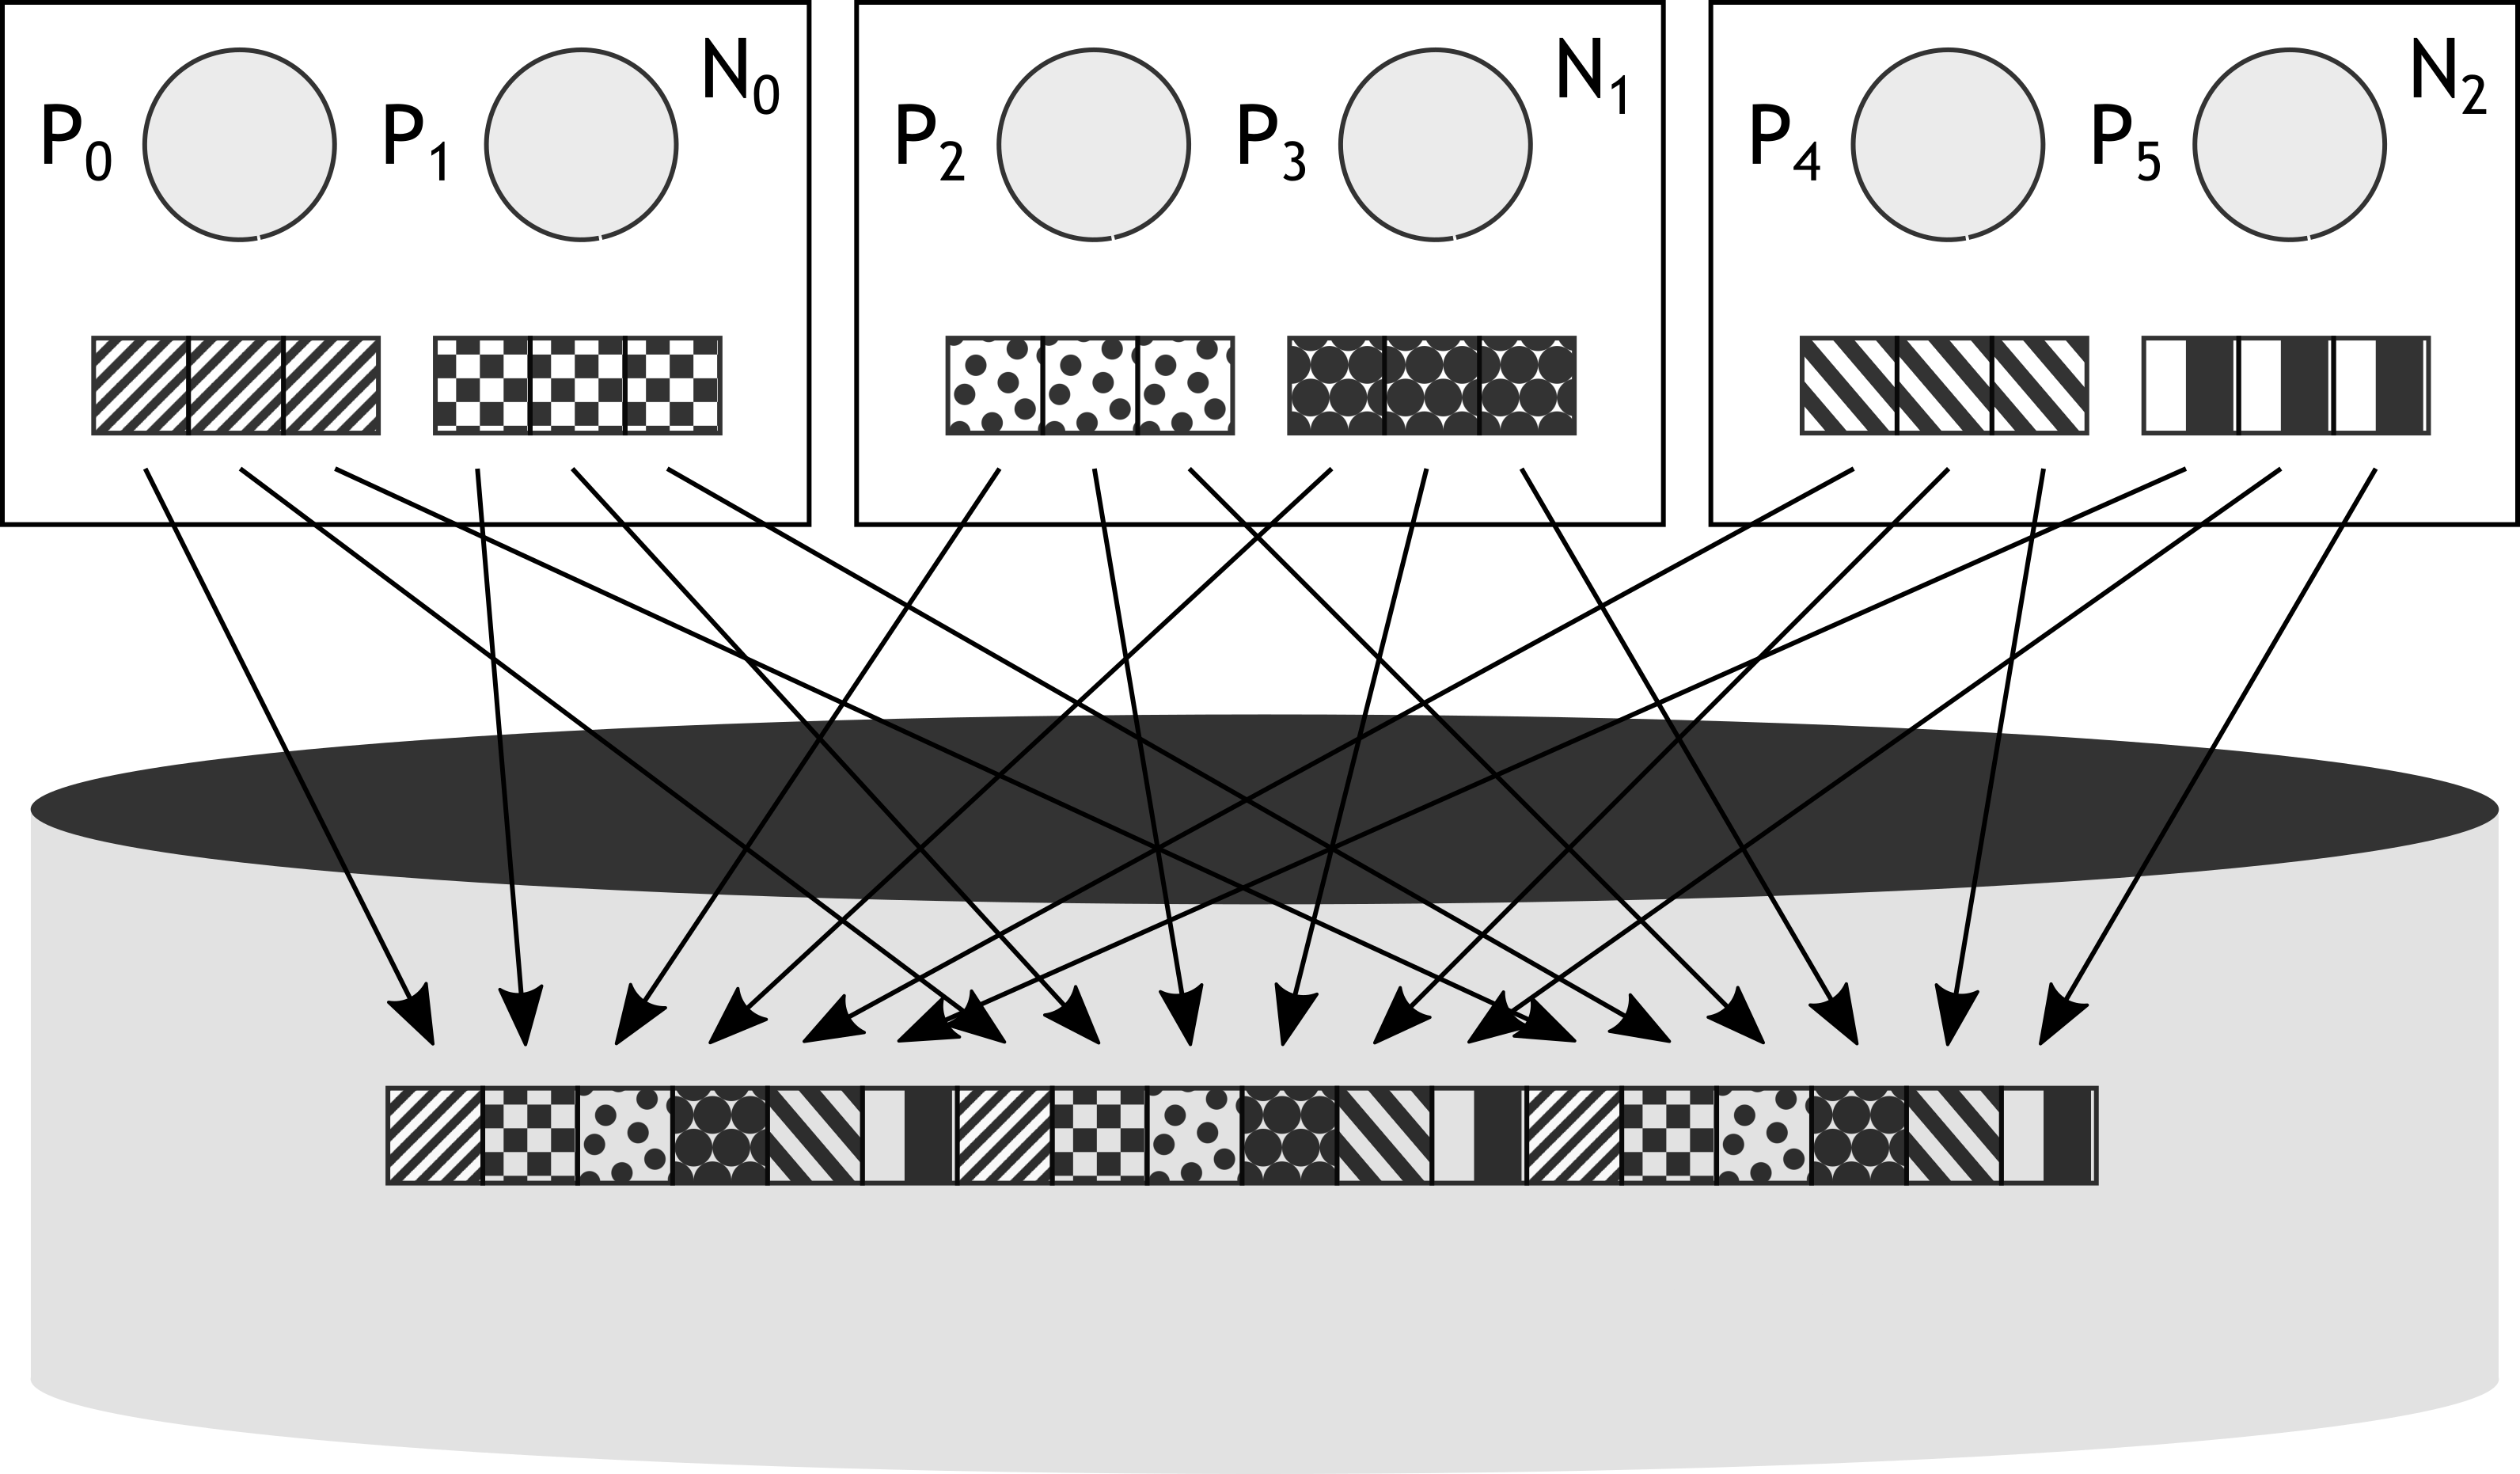
\includegraphics[width=\textwidth]{figures/checkpoint-n-1}
  \caption{N-1 strided pattern.}
  \label{figure: checkpoint-n-1}
  \end{subfigure}
  \caption{Common checkpoint patterns in HPC.}
  \label{figure: checkpoint}
\end{figure}

The N-N and N-1 checkpointing patterns just described are shown in Figure~\ref{figure: checkpoint}. These try to address different performance bottlenecks in parallel file systems, but frequently they just trade one for another. 
For example, in large scale applications composed by thousands of concurrent processes, the adoption of a N-N pattern can alleviate the single shared file locking contention, but requires the creation in the same directory of a 
corresponding number of files to dump each process state. Parallel file systems typically partition the namespace across multiple metadata servers for better performance~\cite{Patil2011}. However, the namespace partitioning is 
often done at the mount point granularity. This causes N-N patterns to overwhelm metadata servers with a storm of file creates, degrading performance. The namespace partitioning also leads to distributed metadata operations that 
have to be handled carefully by the metadata protocol~\cite{Sinnamohideen2010}~\cite{Congiu2012}.
N-1 patterns overcome this problem by using a single shared file for checkpointing, but because scientific codes often write small amounts of non-aligned data, this results into an increased contention on the file and, 
correspondingly, in the serialization of writes. 

N-1 patterns are often preferred to N-N patterns because of their convenience. Indeed, data in a shared file is organized to replicate the original input domain layout and it does not depend on the number of checkpointing processes. 
As a result computation can be restarted from the checkpoint with an arbitrary number of processes; visualization tools that need to display partial results to users are also advantaged because they only need to access one file instead 
of reconstructing the original domain from many small segments.

So far we have implicitly talked about user-level checkpointing in which writes are directly performed by the application. Different user-level checkpoint libraries have been developed over the years~\cite{Bent2009}
~\cite{Frings2009} \cite{Moody2010_2}~\cite{Ansel2009} to improve performance. A system-level approach, that does not require the direct involvement of the application, is also possible~\cite{Wang2007}. In this case, the entire memory 
of every node in the system is dumped to the file system at predetermined intervals. This is, of course, much more expensive because a larger amount of data and system information needs to be written as further studies have
demonstrated~\cite{Kaiser2016}. One additional challenge is the capturing of system information that includes descriptors of open sockets and files, as well as the state of transient network messages. A solution to the problem, that 
makes use of resource virtualization, has been proposed by Arya et al.~\cite{Arya2016}. However, user-level checkpointing still remains the preferred choice, especially when moving to extreme large scale systems.

\section{Memory Technologies}\label{section: mem-tech}
Current compute systems are based on the Von Neumann architecture in which CPU and memory are integral components of the system while storage is relegated to peripheral and accessed through the I/O subsystem using many 
different layers of software (e.g., file system interface, block layer, device drivers). Because external storage typically relies on mechanical devices, such as hard disk drives, that are notoriously much slower than DRAM 
memories, I/O has become the main bottleneck for many applications. As a results there has been a huge effort in terms of research and development of dedicated parallel file systems and I/O middleware solutions that try to 
bridge the performance gap between compute and storage. Historically these solutions have worked out well for specific workloads but they are not resolutive for the problem. Furthermore, the I/O gap is widening and software 
components alone cannot address the requirements of future leadership class systems. Figure~\ref{figure: io-gap} shows the gap between the different memory components in today's systems.

\begin{figure}[!htb]
\centering
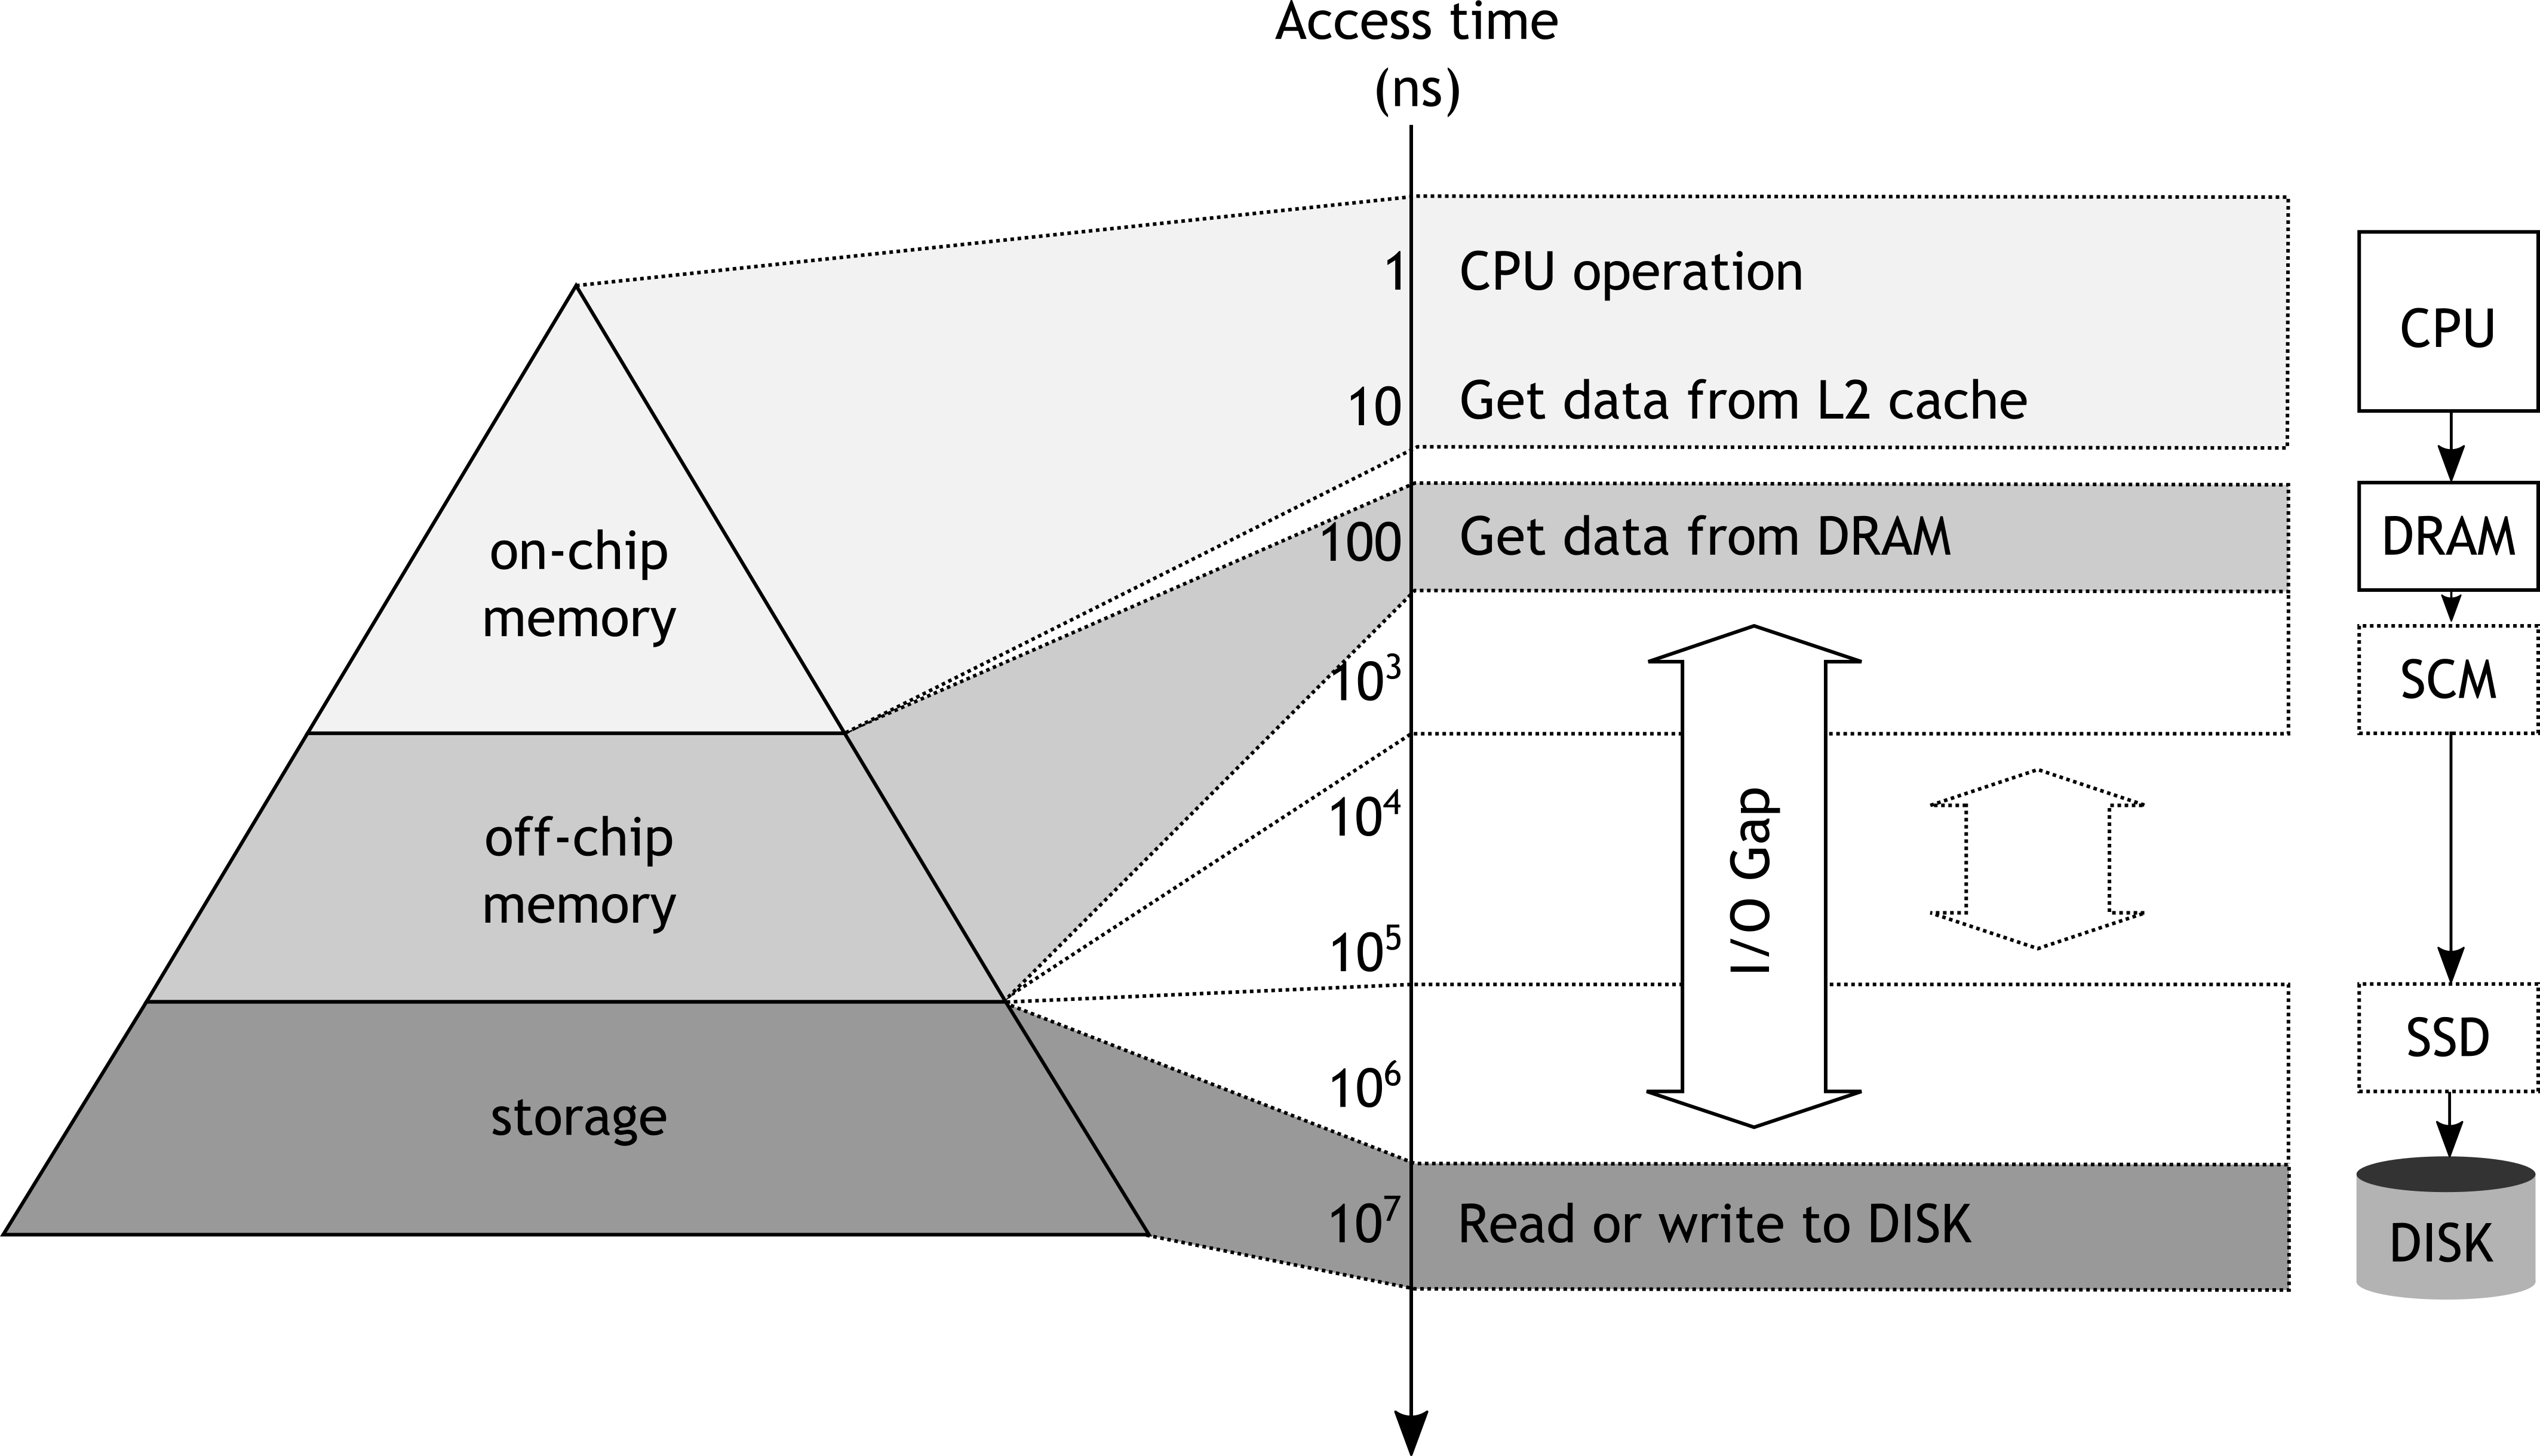
\includegraphics[width=0.9\textwidth]{figures/io-gap}
\caption{Classical memory hierarchy in a standard computer. In the figure the dashed boxes represent existing and emerging solid state devices like SSDs and SCMs.}
\label{figure: io-gap}
\end{figure}

As we can see from the figure, DRAM access times are in the order of hundreds of nanoseconds while disk access times are in the order of tens of milliseconds, a hundred thousand times higher than DRAM. In this section 
we look at existing and emerging mass memory technologies. Some of these technologies, like \textit{flash memories}, have better performance than spinning disks but are still accessed using a block based interface and 
for this reason are a good candidate for implementing a faster storage tier between DRAM and HDDs. Other technologies, like \textit{storage class memories} (SCMs), have performance that approach DRAM and are also byte 
addressable; therefore, they can bring the density and non-volatility of storage media into memory land, providing a good candidate to either replace or sit next to DRAMs.

\subsection{Magnetic Disks}
Hard disks are the most used mechanical storage components for persistently storing data in a computer. Data in hard disks is organized into sectors (elementary transfer units), dislocated on the surface 
of a magnetic disk (or platter). Hard disks can have many platters arranged into a stack, connected through a spindle powered by an electrical motor. Data in the disk is accessed through magnetic sensors, 
or heads, that are moved over the disk surface to read and write data using a set of mechanically actuated arms. Sectors are further organized into tracks (i.e., concentric strips that can be accessed with 
a single head positioning); the disk spins at high speed allowing the head to visit all the sectors in a track. Finally the set of tracks, from the different platters, that are located at the same distance 
from the spindle is called cylinder~\cite{Ruemmler1994}. Since every platter is paired with a set of heads, one for the lower surface and one for the upper, data on the same cylinder can be accessed at the same time using the 
available heads. Figure~\ref{figure: hdd} shows the described device geometry. Although hard disks could transfer data at the byte granularity, in order to achieve acceptable performance disks use sectors
including multiple bytes (512 bytes most commonly); for this reason hard disks are also called block devices. Another feature of hard disks is that they allow data to be accessed in any order, making them 
another type of random access memory like DRAM.

\begin{figure}[!htb]
  \centering
  \includegraphics[width=0.7\textwidth]{figures/hdd}
  \caption{Schematic representation of the components of a hard disk drive.}
  \label{figure: hdd}
\end{figure}

Data access time in HDDs is governed by the mechanical parts that compose the device. The two main contribution in this sense are: \textbf{(a)} the \textit{seek time}, accounting for the time needed to position 
the heads above the track where data will be read or written; and \textbf{(b)} the \textit{rotational delay}, accounting for the rotation time needed to bring the desired sector under the disk head. Additionally 
there is also the \textit{transfer time} accounting for the speed at which data can be read or written and the \textit{queuing time}, accounting for how long a request waits before being served. The 
\textit{controller time} is typically much smaller than the other contributions and is thus ignored here.

As an example, a typical hard disk for desktop applications can have an average seek time of 9 milliseconds, a rotational speed of 7200 RPMs (120 revolutions per second), and a sustained transfer rate of up to 300~MB/s
\footnote{Values reported for the Seagate Barracuda SATA drive, available at \url{http://www.seagate.com/staticfiles/support/disc/manuals/desktop/Barracuda\%207200.12/100529369h.pdf}.}. We can determine the average 
rotational delay from the inverse of the rotational speed as $T_{rot} = \frac{1}{120}\times\frac{1}{2} = 4.16 ms$. The transfer time depends on how long it takes for every sector to transit under the disk head. This 
figure can be determined as $T_{trans} = \frac{512 B/sect}{300 MB/s} = 1.62 \mu s/sect$. If we ignore the queuing time and assume every request is served immediately, the average access time for transferring 2048 
sectors ($N_{sect} = 2048$), or 1~MB, in the considered disk is 16.4~ms, as given by plugging the previous values into Equations~\ref{formula: disk-access-time}.

\begin{equation}\label{formula: disk-access-time}
T_{disk} = T_{seek} + T_{rot} + N_{sect} \times T_{trans}
\end{equation}

The result of 16.4~ms corresponds to a throughput of about 60~MB/s, that is much lower than the 300~MB/s reported by the manufacturer. This is because 300~MB/s is the maximum throughput that can be achieved by the 
drive when reading sequentially. By transferring a large data segment from the drive the impact of head re-positioning can be minimized, on the contrary transferring many small data segments involves several head 
movements that end up dominating the transfer time.

Equation~\ref{formula: disk-access-time} can be replaced into Equation~\ref{formula: io-time} to determine the total average data access time in a distributed storage system.

\subsection{Solid State Drives}
Hard disk drives have dominated the mass storage device market for decades. In 1984 Fujio Masuoka invented the \textit{flash} technology~\cite{Masuoka1984} that today is at the base of modern \textit{solid state drives} (SSDs). Unlike HDDs, 
solid state drives have no moving mechanical parts. Because of this characteristic SSDs are faster and more reliable than HDDs. However, as we will see, the flash technology makes the design of SSDs a challenge.

Data in SSDs is stored inside flash cells. A flash cell can be built using a floating gate CMOS transistor, which represents information as electrical charge trapped inside the dielectric between the channel and the gate. There are 
different types of cells based on how many bits are stored. \textit{single level cells} (SLCs) store only one bit, \textit{multi level cells} (MLCs) store two bits, while \textit{triple level cells} (TLCs) store three bits. 
SLCs are more reliable and have better performance among all and thus are also more expensive. Flash cells are organized into larger units called \textit{pages}, typically 8 or 16~KB in size, and pages are further grouped 
into \textit{erasure blocks}, using a NAND gate configuration. Data can be read and written from and to the flash chip at the page granularity. Nevertheless, a page cannot be re-written unless it is erased first. Unfortunately, 
the flash chip cannot erase single pages but has instead to erase all the pages inside a block. %For this reason some of the pages in the block may need to be copied to DRAM or another set of pages in the chip before the block can be erased. 

Normally read operations are quite fast because the value of the electrical charge in the cell can be retrieved easily (in the order of tens of microseconds). Write operations are typically more expensive because pages 
have to be erased before they can be programmed (in the order of hundreds of microseconds). Additionally, erasing a block causes a wear out of the device that has a limited number of erase/programming cycles. These two 
elements are important aspects that have to be considered when designing a solid state drive based on the flash technology. Figure~\ref{figure: flash-ssd} shows the high-level architecture of a flash based storage device 
as we have just described it.

\begin{figure}[!htb]
\centering
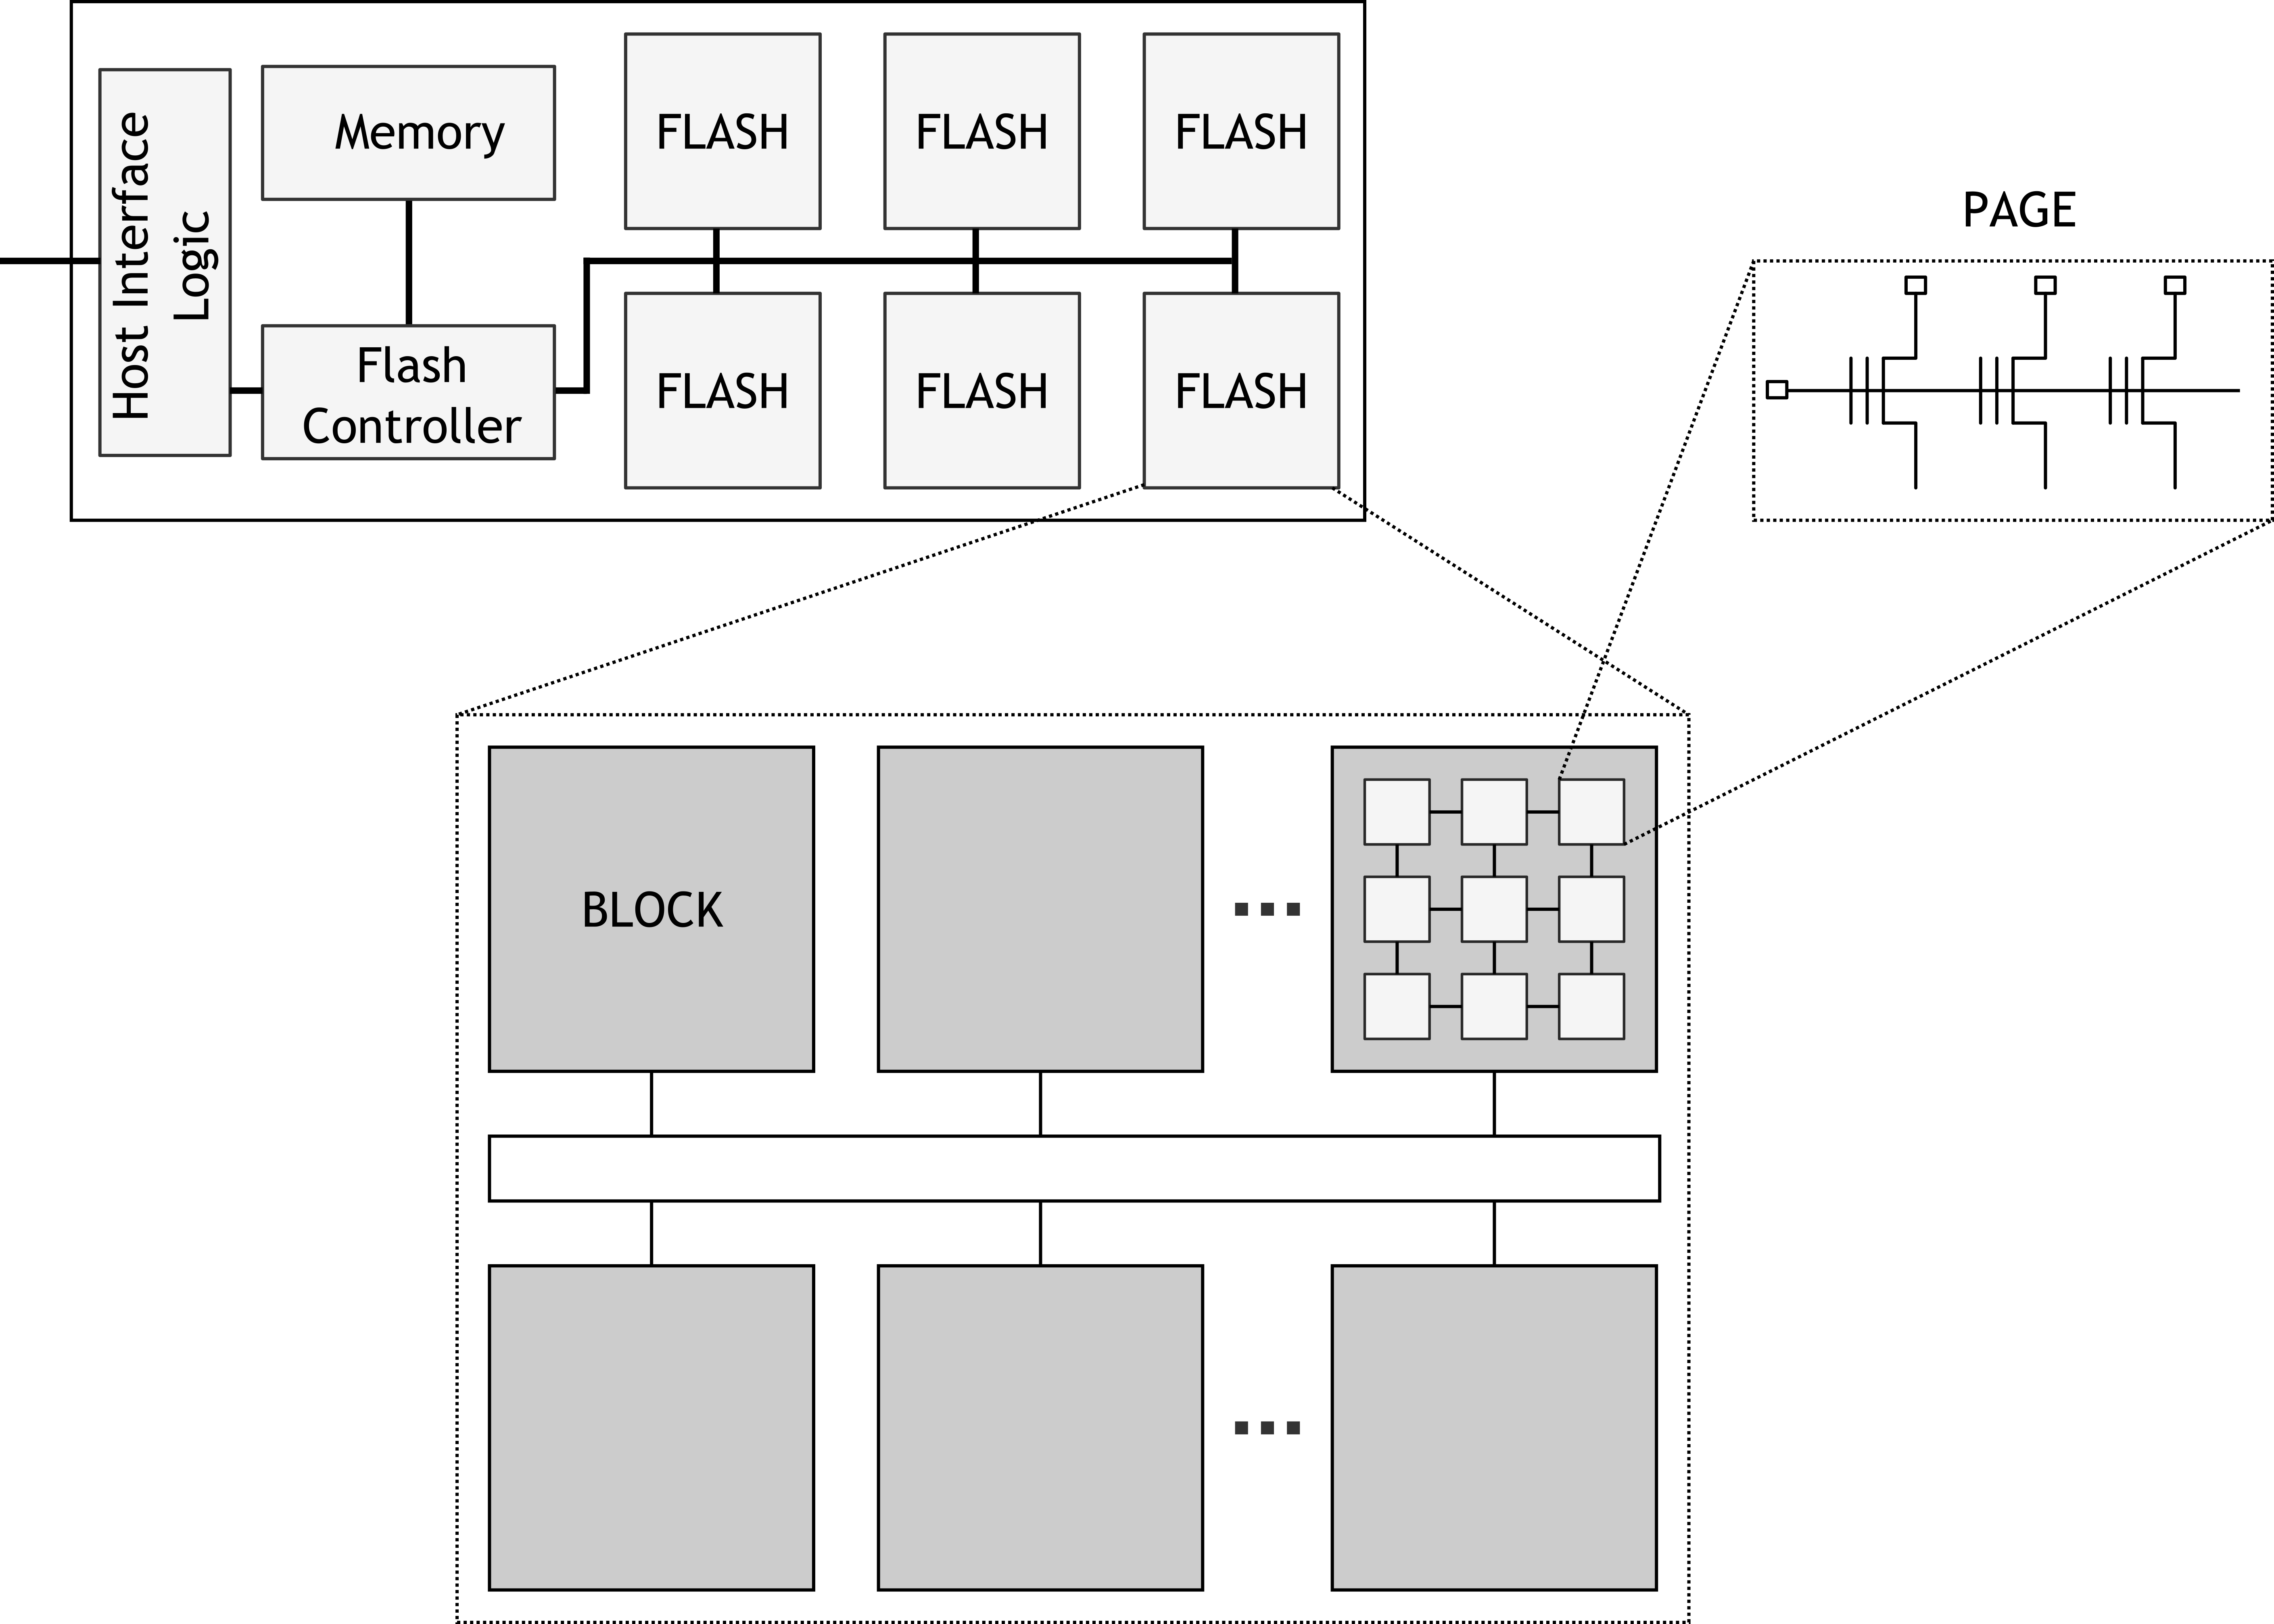
\includegraphics[width=0.9\textwidth]{figures/flash-ssd}
\caption{High-level architecture of a flash based solid state drive.}
\label{figure: flash-ssd}
\end{figure}

A solid state drive is composed of many flash chips, some memory for temporarily storing data read and written to the device, a flash controller and a host interface (SATA for commodity SSDs, PCIe for enterprise SSDs). Most 
of the design effort in this class of devices goes into the flash controller, also called \textit{flash translation layer}, or FTL. The FTL makes the flash chips in the SSD appear externally like a block device, exactly like 
a standard HDD. This means that users can still reference data in the device using logical block numbers and the FTL will convert, or map, these onto addresses in the flash chips.

When a page is updated, the FTL reads it from the target block, applies the changes in memory and writes the updated data to a new page. When all the pages in the block are full the FTL moves to a fresh block; this time, along
with the updated page it also copies all the pages in the old block (while this is selected to be erased later on). Since the erasure of the block is the most time consuming operation (in the order of milliseconds), blocks
are not erased immediately but are instead marked for erasure. Subsequently, a garbage collection algorithm gathers all marked blocks and erases them. During the update of a page it is also important to decide where data from
one block is moved. Because blocks have a finite number of erase/program cycles, it is crucial that all of them receive a similar number of erase/program operations. This is called wear leveling and is also responsibility of
the FTL. In this sense it is worth to mention the work done by Margaglia and Brinkmann to improve SSDs endurance (as well as performance) by doing write in place updates to pages~\cite{Margaglia2015}.

We have seen as for HDDs read and write performance are quite similar and we have also seen that for flash chips this is not the case, with write operations being ten times slower than reads (tens of microseconds for reads
against hundreds of microseconds for programs). This performance issue is commonly addressed by the SSD writing in parallel to multiple flash chips. However, the FTL logic and the disk block interface limit the device 
performance. As an example, a modern Samsung 6~Gb/s SATA SSD can have sequential read and write performance of 540~MB/s and 520~MB/s, respectively\footnote{Values reported for the Samsung 805 Evo SSD, available at 
\url{http://www.samsung.com/semiconductor/minisite/ssd/downloads/document/Samsung_SSD_850_EVO_Data_Sheet_Rev_3_1.pdf}.}, while a PCIe Samsung SSD can have sequential read and write performance of $3,500$~MB/s and 
$2,100$~MB/s respectively\footnote{Values reported for the Samsung 960 SSD, available at \url{http://www.samsung.com/semiconductor/minisite/ssd/downloads/document/Samsung_SSD_960_PRO_Data_Sheet_Rev_1_1.pdf}.}. The performance
difference is due to the higher transfer rates of the PCIe interface.

Because PCIe SSDs can perform an order of magnitude better than HDDs but are still inferior to DRAM, they can be used as additional block based cache layer placed between DRAM and hard disks. This is exactly the type 
of application these devices are finding in high performance storage systems.

\subsection{Storage Class Memories}
Storage class memories promise to bring together the characteristics of permanent storage (capacity and non-volatility) and memory (low latency and byte addressability) in the same device, providing at the same time better 
power efficiency than SRAM and DRAM technologies. Indeed, conventional main memories are volatile and require a permanent source of energy to maintain, or periodically restore, the integrity of the data. This last 
characteristic makes SCMs particularly attractive for the deployment in large scale leadership class machines, that can have several Terabytes of main memory. 

Different technological solutions have been proposed for storage class memory devices, including \textit{spin-transfer torque magnetic RAM} (STT-MRAM)~\cite{Wang2013}, which provide access times comparable to DRAMs but are
less dense; \textit{resistive RAM} (RRAM)~\cite{Zhang2015}, which are a little slower than STT-MRAM but more dense; \textit{3D XPoint}, which resulted from the collaboration between Micron and Intel; and \textit{phase change 
memories} (PCMs)~\cite{Breitwisch2008}. SCM devices based on these technologies can be addressed at the cache line level like DRAMs and can thus be employed as \textit{non-volatile main memories} (NVMMs) placed directly on 
the memory bus using a \textit{non-volatile DIMM} (NVDIMM) interface~\cite{Lee2009}.

The availability of NVMM opens up a new range of alternatives for implementing persistent data storage solutions. For example, so far file system developers had to rely on magnetic disks to store files. Because hard disks are 
slow block devices, disk based file systems interfaces and data consistency semantics have been defined accordingly. As we have seen in the introduction of this chapter, POSIX enforces atomicity and consistency but not durability. 
Durability is deliberately avoided because of the cost of committing updates to disk. Similarly, data accesses are typically block aligned in both offset and size to improve transfer rates. These design choices no longer hold 
for NVMM based file systems~\cite{Xu2016} which can access data fast and at the cache line level. Because data can be stored permanently in the NVMM, file systems no longer need to use the page cache to coalesce updates into large 
batches, thus avoiding the extra copy operation. Direct access to the NVMM is provided by the operating system using \textit{direct access extensions} (DAX) or \textit{execute in place} (XIP).

A problem with implementing file systems in main memory comes from the consistency requirements that are normally imposed upon update operations and that guarantee correctness of applications performing I/O. In this case, CPUs 
can rearrange the order of operations to improve performance, potentially breaking consistency in the case of a system failure. To avoid this, file systems in main memory have to explicitly enforce the flushing of CPU caches to 
respect ordering but, at the same time, adding considerable overhead. In order to ensure atomicity, NVMM based file systems have to employee journaling mechanisms that perform efficiently on the new hardware. In fact, although 
SCMs can effectively bridge the gap between storage and compute, they will just move the bottleneck from the device to the system software and applications, which performance will be no longer dominated by storage latency
~\cite{Katzburg2016}.

\section{Caching}\label{section: caching}
In the previous section we have introduced hard disk drives and discussed the performance gap between storage and compute. We have also seen that high performance storage systems improve performance of disk based file systems 
by providing independent parallel data paths from clients to storage devices. Another effective way to improve performance is to exploit common access pattern characteristics to intelligently move data from storage to main memory. 
Many computer programs exhibit data locality characteristics both in space and time. For example, during normal execution the CPU will load instructions from a binary file stored on disk and execute them in sequence, from the first 
to the last. Because file systems try to minimize disk access time by placing data contiguously on the device, the corresponding instructions are also spatially contiguous. Moreover, most programs repeatedly perform the same set of 
instructions inside a loop. These characteristics can be exploited by the operating system to intelligently move data from disk into a region of DRAM to serve it more rapidly to applications, thus reducing I/O stall time. To this 
end the Linux kernel uses a dedicated area of main memory called \textit{page cache}~\cite{Bovet2008}. The page cache buffers data from storage devices using the file system block granularity and normally adopts the same block 
size also for pages.

In order to understand how the page cache can improve I/O performance let us consider a simple read example. When the kernel receives a read call, it first tries to locate the requested data in the page cache. If data is not in the 
page cache, the read call causes a \textit{page miss}, which triggers a disk operation to retrieve it from the external storage device. To handle the disk operation, assuming there is enough space available in the cache, the kernel 
allocates a new page and instructs the DMA controller to fill it with data from disk. When the DMA controller has completed the transfer, it notifies the kernel using an interrupt. At this point the kernel copies the freshly read 
data from the page cache into a user buffer in the program address space and returns control to it. The additional copy from page cache to user buffers adds latency but because disk I/O is much more expensive than a memory copy,
the cost is hidden in the total data transfer. Once data is in the page cache, future references to it can be served faster without involving the external storage device. 
Similarly, the cache can be also used to hide disk access to write operations. In this case data updates are applied to the page cache and are committed to disk later on, while control is immediately returned to the application. 
Cached data can be committed to disk either explicitly, using an appropriate system call (e.g., \texttt{flush()}) or by the kernel after some time has elapsed. The length of this interval depends on several parameters, like the 
amount of available memory, the number of \textit{dirty pages} (i.e., the number of uncommitted updates in the cache), and so on.

File caching is effective in improving performance of local and distributed applications by hiding to them disk latency. However, caching is typically performed at the kernel level and thus does not account for global context in 
distributed codes. Parallel applications have multiple processes that are executed simultaneously in different compute nodes and access the same file concurrently. In this case if caching is done independently by every process, the 
burden of enforcing cache coherency is pushed to the parallel file system which has to grant exclusive locks to processes, ultimately serializing data access. These processes could instead collaborate to cache data as they were a 
single program running on the same physical machine. The advantage in this case is that file system clients can manage data consistency more efficiently without involving the parallel file system. Moreover, by using global context, 
overlapping accesses can be filtered to eliminate duplicated data in the cache. Liao et al.~\cite{Liao2005} have implemented a distributed caching scheme, called collective caching, in the MPI-IO layer~\cite{mpispecs}. The proposed 
scheme takes advantage of the global application knowledge to efficiently buffer data at the user level. Because each file block can be cached only by one client this approach avoids false sharing and thus reduces the interaction 
between the application and the file system lock manager.

\subsection{Readahead and LRU}
In read patterns the locality of reference in the data can be exploited in two ways. First, the kernel can extend the size of a read request to transfer a little bit more data than originally requested, in a process called \textit{
readahead}; because the probability of this data being accessed next is high, a future reference to it can be quickly served from the page cache, completely hiding disk latency to the program. Second, because of the cyclic nature 
of programs, when cache space is scarce pages to be removed, or \textit{evicted}, from the cache are selected among the \textit{last recently used} (LRU).

\begin{figure}[!htb]
\centering
\includegraphics[width=0.8\textwidth]{figures/readahead}
\caption{Effect of readahead on a program that reads sequentially blocks of data from a file in the disk. In the example, every data block $Blk_i$ is read and afterwards processed $P(Blk_i)$ by the application.
Readahead can merge the reading of two adjacent blocks amortizing the disk latency.}
\label{figure: readahead}
\end{figure}

To further clarify the concept of readahead let us consider the example shown in Figure~\ref{figure: readahead}. In the example, the disk access latency is broken down into two components: the head positioning, given by the 
sum of seek time and rotational delay, and the data transfer time. Because readahead can enlarge the request size, two blocks of data can be read with a single head positioning, saving two seek operations to the application.

Although locality based heuristics can be useful to improve the performance of many programs, they cannot be applied to all the use cases. For example, codes might exhibit non-sequential file access patterns. A readhead 
strategy in this case would bring into the page cache data that has little chances to be referenced. Not only this does not improve performance but can have harmful effects on the overall system efficiency. In fact, the extra 
requested data is likely to steal disk bandwidth from other requests, and since the physical amount of memory in the system is limited, it will pollute the cache, possibly causing the eviction of more valuable data that will 
have to be fetched again from the disk later on. However, a locality based strategy that takes into account the global application access pattern could be beneficial for some parallel codes. As we have introduced in Section
~\ref{section: hpc-io-sys}, when talking about the small I/O problem, scientific codes often access data using a regular pattern that can be easily exploited to effectively bring data into the cache. This observation is 
explored by Chen and Roth~\cite{ChenR10} whom show that for strided patterns in the pio-benchmark~\cite{shorter2003} locality based heuristics can be still useful when applied to the application's processes as a whole instead 
of considering them independently.

\subsection{Prefetching}
In normal working conditions, data is transferred from disk to page cache in response to a page miss, triggered by a read call. Therefore, disk latency can only be hidden to following page references while the first access will 
always suffer the full I/O latency. Readahead can hide disk latency for data that is spatially local to the current request but is harmful to the performance of applications that do not exhibit such locality. For these applications 
readahead is typically disabled. To overcome such limitations more sophisticated caching strategies have been proposed.

Prefetching is a proactive caching mechanism used to completely hide disk latency to read operations. In this case, data from disk is brought into the page cache before it is actually referenced by a read call and, when needed, is 
served to the application from the cache instead of the disk. The readahead strategy previously described is in fact a special case of prefetching that relies on data locality. In readahead the prefetching request is piggy backed 
onto the original read operation, triggered by a page miss, and targets data that is contiguous to the originally request in disk~\cite{Bovet2008}.

In this thesis we focus on \textit{guided prefetching} strategies because, unlike readahead, data can be fetched at any time and from anywhere in the file. However, when and how much data to prefetch become important parameters that 
need to be carefully evaluated. Indeed, prefetching has to be performed at the right moment and only for the right amount of data in order to bring improvements to the run-time, especially in systems with limited available memory. 
Prefetching too much data, or prefetching it too early, may cause more urgently needed data to be evicted from the cache, forcing the application to fetch it from disk again later on. Contrarily, prefetching data too late adds 
unnecessary overhead associated to the processing of the corresponding system call by the operating system and might even fetch data that was previously evicted because no longer needed.

\begin{figure}[!htb]
\centering
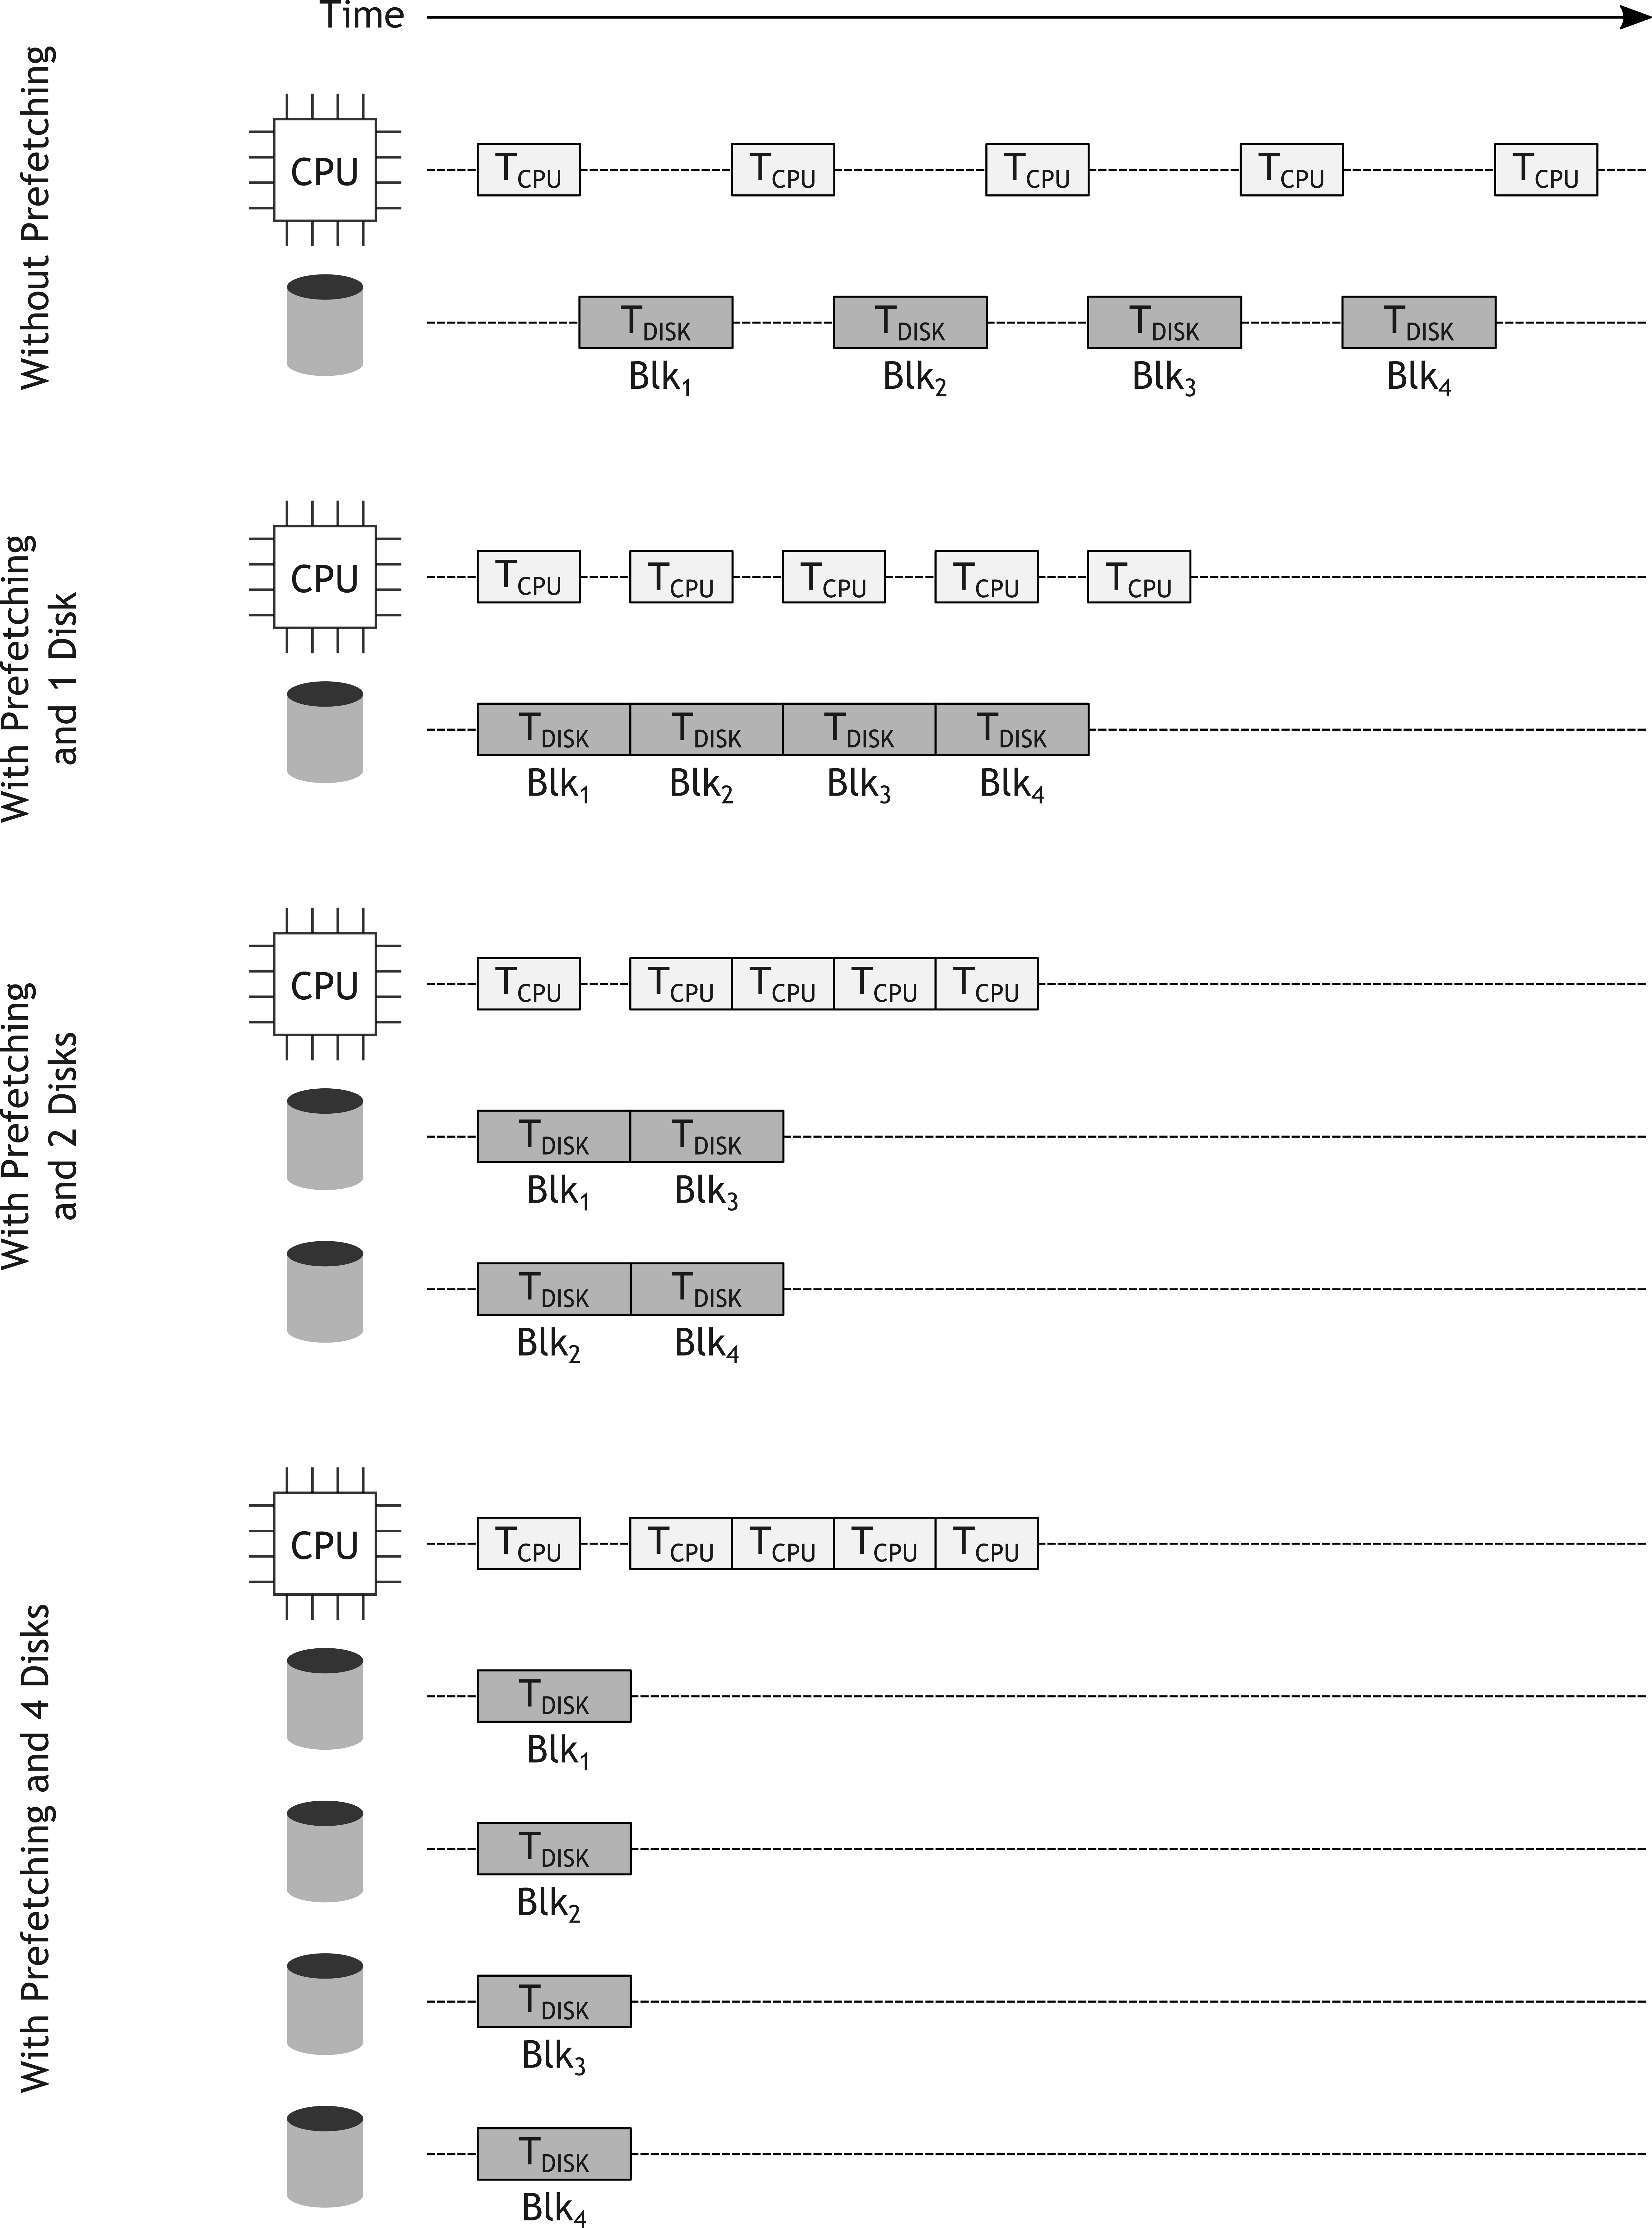
\includegraphics[width=0.8\textwidth]{figures/prefetching}
\caption{Effect of increased storage bandwidth on prefetching performance.}
\label{figure: prefetching}
\end{figure}

Disk bandwidth and memory capacity directly affect prefetching performance. To understand how consider the examples reported in Figure~\ref{figure: prefetching}. We have an application that alternates phases of compute, at the 
end of which some data is read from disk, to phases of data transfer from disk to memory. The performance baseline for the run-time is given by the first case, in which prefetching is disabled. The remaining three cases show 
how run-time behaves when prefetching data from one or more disks. In the first of the three only one disk is used and we can observe that, because the application is I/O bound, the minimum run-time is limited by the total disk 
latency. Increasing the number of disks from one to two doubles the bandwidth and thus the number of blocks that can be transferred at the same time. In this case disk latency can be completely hidden to the application, which 
progresses with no I/O stalls. Further increasing the number of disks from two to four does not add any further benefit because there is no latency left to hide. In general, for disk bound applications like the one considered, 
disk accesses can be completely hidden through prefetching if data is distributed appropriately across, at least, $\ceil*{\frac{T_{disk}}{T_{CPU}}}$ disks~\cite{Chang2001}.

Although higher disk bandwidth can improve prefetching performance by allowing more data to be retrieved in parallel from the available devices, final performance also depends on the amount of cache space; it does not matter if two 
blocks can be prefetched at the same time, unless there is enough space in the cache to host both of them. If cache space is not enough to hold the two blocks, prefetching can degrade I/O performance. This eventuality is shown 
in Figure~\ref{figure: prefetching_2}. When the application begins execution, it immediately issues to the kernel a prefetching request that covers $Blk_1$ and $Blk_2$. The kernel receives the request and initiates two disk transfers,
one per block. Assuming $Blk_1$ is requested first, the kernel allocates a new page and initiates a disk operation to fill it, then it moves to $Blk_2$ and tries to do the same. However, because the only available page is already in 
use for $Blk_1$, it has to wait. Although the available disk bandwidth is enough to fetch two blocks at the same time, the lack of memory space results in the serialization of I/O at the page cache level. Moreover, when $Blk_1$ is 
finally in the cache, its page is evicted to transfer $Blk_2$. While $Blk_2$ is being fetched, the application makes the actual reference to $Blk_1$, which was previously evicted and has to be fetched again after $Blk_2$. The same 
happens for $Blk_3$ and $Blk_4$ later on. This causes a continuous transfer of blocks between memory and disk that increases I/O activity and correspondingly the application execution time.

\begin{figure}[!htb]
\centering
\includegraphics[width=0.8\textwidth]{figures/prefetching_2}
\caption{Effect of limited cache space on prefetching performance.}
\label{figure: prefetching_2}
\end{figure}

Guided prefetching strategies rely on applications access pattern knowledge to timely transfer the necessary file data from disk into the cache. This knowledge can be directly exploited by manually inserting prefetch calls in 
the right place inside the code. However, this requires manual intervention and increases both complexity and programming efforts. Moreover, programmers are often reluctant to make changes to codes that have taken years of 
development to mature to a satisfactory level. Sometimes, the source code is not even available and only the program binaries are at hand. This makes it impossible to manually insert any prefetch call into the code. To overcome 
these problems, automatic and dynamic history-based approaches to prefetching have been proposed. Automatic prefetching can be further divided into \textit{static} and \textit{speculative} strategies, depending on how the 
prefetch requests are generated and added to the application. Dynamic history-based approaches, on the other hand, rely on the analysis of the I/O history to infer when prefetching should be performed; such solutions do not alter 
the application code or binary and delegate prefetch call issuing to an external software component, typically a middleware or the file system itself.

\subsubsection{Automatic Prefetching}
For automatic strategies it is important that prefetch requests are not issued using asynchronous read calls. This is necessary for two reasons; first, read calls are immediately converted by the operating system into data transfers 
from the storage device. However, automatically generated requests are not accurate because they do not consider the dynamically changing system parameters, like memory usage. Therefore, the operating system needs to have some 
flexibility to decide whether or not a request should be actually converted into a disk access; second, read operations are binding, which means that data fetched using a read operation is supposed to be consumed immediately and can 
be changed afterwards. Nevertheless, the basic assumption about prefetching is that data fetching and consumption can be decoupled so that data is brought into the cache ahead of time and consumed only later on, when it is referenced. 
For this reason prefetched data should not be mistakenly changed by the program if the prefetch call is moved ahead of a store to the same memory location by the compiler. To address these issues prefetch hint interfaces are employed. Hints are not 
immediately converted into data transfers and are non-binding, ensuring the correct behaviour of the application, no matter how far ahead in time they are submitted.

\paragraph{Static} prefetching approaches exploit a code analyzer, typically a compiler, to extract access pattern information from the application and identify in which points of the code prefetch calls have to be inserted in order to hide the
latency of a page fault triggered I/O operation\footnote{Here we are implicitly considering automatic static prefetching for applications that access the disk using paged virtual memory and not explicit I/O operations.}. Because static
analysis does not consider dynamic system parameters, the compiler has to take an aggressive approach and inserts a prefetch call every time a page is reused. However, during execution the system might have sufficient memory to keep
the target page in the cache between two consecutive accesses. In this situation, a prefetch call that is automatically converted into a system call for the OS would add no benefit to the execution time; on the contrary, it would add
the overhead for the corresponding system call processing. For this reason static approaches combine compiler inserted hints with run-time and operating system support. The run-time and operating systems collaborate to exchange virtual
memory information and, based on this, the run-time decides whether a prefetch call should be converted into a system call or not. 

Mowry et al.~\cite{Mowry1996} and Brown et al.~\cite{Brown2001} have used compiler inserted hints to improve performance of paged virtual memory for the applications contained in the NAS parallel benchmark suite~\cite{Bailey1991}. 
The run-time and the operating systems share virtual memory information using a memory page, which is allocated at application start up when this registers with the OS. The shared memory page contains a bit-map describing used and 
unused pages in the address space. When the run-time system receives a prefetch call for a page that, according to the bit-map, is already in the cache it drops the request, avoiding to incur into unnecessary system call overhead. 
The bit-map is updated by both the run-time and the operating system as the application progresses.

In a multiprogramming environment, main memory is shared among several applications. If on one side, prefetching has the potential to improve the performance of out-of-core applications, on the other side it might negatively impact 
the performance of others, especially interactive codes that can be idle for a long time. For such codes inactive pages would be sacrificed to prefetch requests of more memory intensive codes, degrading their responsiveness. To 
improve memory management in multiprogramming environment, Brown and Mowry~\cite{Brown2000} have exploited \textit{release} hints to explicitly sacrifice pages that are not expected to be reused again, or are expected to be reused 
but, due to insufficient memory, are going to be selected for eviction by the OS. Once again, because static analysis does not consider dynamic conditions, release hints are aggressively inserted for every page that is referenced 
multiple times. The run-time system compensates the static behaviour by dynamically adjusting the hints to the changing memory conditions. For example, if a release hint is issued for a reused page, the run-time checks whether the 
available memory is sufficient to keep the page in the cache. If it is, the release hint is discarded, otherwise it is forwarded to the operating system.

Although compiler inserted hints can automatically generate prefetch calls and insert them in the code, the required code analysis in the compiler has to make simplified assumptions that affect the accuracy of the technique.

\paragraph{Speculative} prefetching issues prefetch calls to the underlying run-time or operating system by pre-executing application code. In order to move ahead in the code and find out about future reads, the program makes hypothesis about 
the value of dynamic variables. If the speculation is correct the technique can effectively predict what data will be accessed next and timely issue a hint for it. Speculative prefetching can be implemented using a compiler or, if 
the source code is not available, a binary modification tool. In both cases the original code is extended with a speculative thread that executes a modified copy of the original code, also called \textit{shadow} code. In the shadow 
code read calls are replaced with prefetch hints and can be executed either using the spare CPU cycles resulting from an I/O stall of the main thread or using a further physical thread to run in parallel with the main thread. 

One problem with speculative execution is that main and speculative threads share the same address space. Speculative execution might thus alter the original program behaviour by changing code or data used by the original program. 
This can cause side-effects that are visible outside the process, impacting the whole system behaviour, or can inadvertently produce data values that cause the program to deviate from normal execution.

Chang and Gibson~\cite{ChangG99} proposed \textit{SpecHint} as binary modification tool to implement speculative execution. In SpecHint the shadow code is generated appropriately from the original binary to address the previously 
described problems and is executed during I/O stalls of the main thread using the spare CPU cycles. In SpecHint, load and store operations that involve shared variables are preceded by additional checks to make sure that memory 
accesses are redirected to a private copy of the original variable (copy-on-write). External side-effects are avoided by cleaning out the shadow code of every system call that is not a hint, a \texttt{fstat()}\footnote{Returns
information about an open file.} or a \texttt{sbrk()}\footnote{Moves the top address of the heap up and down. This system call is used by libc functions such as malloc and free when allocating and deallocating dynamic memory.}.
Finally, automatically inserted exception handlers make sure that inappropriate data values do not disturb normal execution. Whenever an exception is encountered speculative execution is halted and is resumed only when the original 
thread blocks on a read call. In order to ensure that speculative execution does not fall behind the main thread, references to issued hints are kept and compared with following read calls. If a read call is not paired by a 
previously issued prefetch, speculation is not working as expected and should be realigned with the original execution. SpecHint does not use any special run-time to handle hints but fully relies on operating system support, 
implemented by replacing the default buffer manager with the TIP manager~\cite{Patterson1995}.

While SpecHint modifies the application's binary to pre-execute the shadow code and issue prefetch calls, Chen et al.~\cite{ChenBSTG08} have applied the same idea to MPI programs using a source-to-source compiler. Additionally,
instead of exploiting unused spare CPU cycles resulting from I/O stalls, the parallel approach takes advantage of the additional physical threads to access data concurrently with the main thread. To avoid the pre-execution thread 
to change memory regions shared with the main thread a variable renaming technique is employed. This is more expensive in terms of memory requirements compared to the copy-on-write technique used in previous work but is not that 
critical in parallel machines with large memories. The problem of non-binding hints, previously described in the context of automatic prefetching, is solved by marking write operations as synchronization points.

Every time the pre-execution thread encounters a write call it waits for the main thread to arrive before continuing with execution. The drawback is that the amount of progress that can be made is limited. To alleviate this effect 
the authors observe that dependencies are critical only for RAW (Read After Write) operations. Therefore, when the speculating thread encounters a write call it registers its range (dirty range) and continues with execution. When 
the following read call is encountered its range is checked against the dirty range and if the two do not overlap speculation can continue; otherwise, delayed synchronization is performed. Hints are issued by the modified application 
to the underlying run-time system, that is represented by the ROMIO MPI-IO implementation. The used ROMIO version includes a collective caching infrastructure~\cite{Liao2005} and a prefetching library that manages prefetch calls. 
Because the cache is implemented in the run-time library, there is no required support from the operating system.

\subsubsection{Dynamic History-based Prefetching}
While automatic prefetching mechanisms are suited for random access patterns that cannot be predicted by analyzing the history of the application, dynamic history-based prefetching can be applied to applications that exhibit 
some correlation in their access pattern. In order to answer the questions of when and how much data to prefetch, history based solutions accumulate I/O pattern knowledge and use it to take decisions. Such knowledge includes 
temporal behaviour, some times captured by looking at the inter-arrival time of read requests, as well as spatial behaviour, frequently captured by looking at what blocks in the file are referenced and in which order. The 
accumulated knowledge can then be used to train a neural network or to build a mathematical model to guide prefetching in the underlying run-time or operating system.

Tran and Reed proposed a time series modeling system called TsModeler~\cite{TranR04}. TsModeler receives inter-arrival access pattern information from the underlying PPFS2 file system framework~\cite{Simitci1999}, computes the model 
parameters and feeds them back into PPFS2. The file system is responsible for building the spatial model, interpreting the time series coefficients and combine the two models to guide data prefetching. In TsModeler time series 
analysis is performed to build a mathematical model of the inter-arrival time of read requests using an \textit{autoregressive integrated moving average} (ARIMA)~\cite{Newbold1983} for the model's coefficients. The built model predicts
when prefetching should be performed, typically before the actual request for the data arrives, but not too early to avoid other needed data to be evicted from the cache before it is referenced. PPFS2 employes Markov models to 
predict the spatial distribution of future accessed file blocks. Markov models can represent blocks as rows and columns of a matrix and the probability of accessing one block after the other as the matrix values. The Markov model 
can be either built online, for patterns that have data dependencies, or offline, for patterns that repeat.

%In their approach they distinguish between different types of interarrival patterns which are a reflection of the internal structure of the originating program. Seasonal (periodic) patterns are produced by codes with nested 
%loops in which I/O is an other loop operation while stationary and non-stationary are characterized by an inter-arrival time that oscillates around an average time and by an increasing or decreasing inter-arrival time, 
%respectively. 
%In order to detect the type of interarrival pattern and compute the model parameters they use the autocorrelation function and the partial autocorrelation function. If the autocorrelation function decays exponentially or 
%sinusoidaly the pattern is stationary. If the autocorrelation function has peaks at regular intervals the pattern is seasonal and might also have some traces of non-stationarity. Because stationary patterns can be represented 
%using an Autoregressive Moving Average (ARMA) model the authors reduce non-stationary and cyclic pattern to stationary by performing one or more differencing operations and doing so building an ARIMA model which includes 
%differencing. For non-stationary components a differencing of step 1 is typically used (d). For seasonal components the differencing step is the period of the repetition S and the number of differencing is D.
%In order to produce forecasts the parameters of the transformed series must be changed to reverse the transformation process to recover forecasts for the original series. Integration reversals traverse the RDI chain upward.
%They use the ARIMA model to predict prefetching events and use PPFS2 to extract the spatial model (MM) of the pattern. Markov model can be either done online for patterns that have data dependencies or offline for patterns 
%that repeat.
%In order to prefetch the right amount of blocks at the right time  prefetch builder that considers both time series model and markov models. To decide how many blocks to fetch they define a measure for disk congestion. In practice 
%the cumulative time required to fetch all the blocks must be smaller of the total interarrival time for the last targeted block.
%Having everything in place they test the accuracy of both time series model and the corresponding prefetching performance on three applications: PRISM, a numerical simulation application, ESCAT, a low temperature plasma modeling 
%code, and Cactus, a numerical relativity code.
%The time series model achieves an accuracy of 82\%, 90\% and 85\%, respectivelly for the three above mentioned benchmark applications. For cactus the run-time reduction using prefetching increases when increasing the number of 
%cycles in the application because the modelling requires some initialization time before starting to generate accurate predictions.

He et al.~\cite{HeBTAGGMCS13} have observed that many data intensive codes exhibit regular access patterns over multiple runs. To improve the performance of such patterns they have proposed a caching and prefetching framework built 
in the PLFS file system. The resulting PLFS modification can detect recurrent access patterns and use them to guide data prefetching through a dedicated thread. Byna et al.~\cite{Byna2008} also targeted regular access patterns to 
build a mathematical representation of the application I/O behaviour, called I/O signature, and use this representation to guide prefetching during following runs. The prefetching and caching functionalities in this case are 
implemented at the MPI-IO level inside the ROMIO middleware. 

The solutions discussed so far rely on low level access patterns information (i.e., offset and length pairs of I/O requests) to build the knowledge required to guide I/O prefetching; however, this type of low level information carries 
little or no information about the use of data made by the application. High-level I/O libraries, such as HDF5~\cite{Folk99} and netCDF, provide better insights on the data usage pattern because they naturally carry semantic information 
including, temporal sequence of data accesses, combination of data (e.g., two variables that need to be fetched from disk to be combined and produce some results), and relations between data and computational phases (e.g., read of 
variables that are used in computation and produce a result variable that is written to disk). Basing on these observations, He et al.~\cite{HEST12} have exploited high-level I/O behaviour in netCDF to build data dependency graphs that 
are afterwards used by their PnetCDF~\cite{li2003} framework to match the run-time I/O behaviour with the pre-stored patterns and perform data prefetching.

\subsubsection{Manual Prefetching}
Manual prefetching refers to the insertion of prefetch calls inside the application's source code by the programmer; additional support is normally provided by the run-time and operating system for managing the issued hints. 
Patterson et al.~\cite{Patterson1995} have proposed a hint interface and a customized buffer manager. The buffer manager has to balance the benefit of prefetching data blocks from disks with the cost of evicting existing blocks. 
Because the amount of memory at disposal is limited, the buffer manager delays block fetching just before the corresponding data is referenced. VanDeBogart et al.~\cite{VanDeBogartFK09} take advantage of larger memories to implement 
a greedier prefetching strategy that fetches as many blocks as possible in a single batch. The proposed \textit{libprefetch} and kernel extensions advocate to maximize I/O throughput reducing seeks rather than overlapping disk and 
CPU activity to hide disk latency. Whenever possible, seek cost is reduced by filling the gap between two requests with the data in between, using a technique similar to the \textit{data sieving} mechanism supported by some parallel 
I/O middleware.

In this thesis we pursue the same approach and take advantage of large primary memories in HPC compute nodes. We use programmer I/O knowledge to drive prefetching of data into the cache and use data sieving to minimize the effect 
of disk seeks on performance. We do this by relying on the file system prefetch interfaces provided by the Linux \textit{virtual file system} and the GPFS file system. Unlike libprefetch that synchronously transfers a large number of 
blocks in a single batch from the disk we try, as much as possible, to issue prefetch calls to the kernel asynchronously using an additional thread. 

\subsection{Write Behind}
In previous sections we have seen how caching can be useful to reduce I/O stalls when accessing frequently requested data. We have also seen how caching can be used to preemptively fetch disk data into memory, hiding partially 
or even completely I/O latency to applications. Although so far we have focused on read access patterns, caching can also be useful in write operations using a \textit{write-behind} strategy. In write-behind data updates are not 
immediately committed to disk. In fact, as we have mentioned earlier when discussing file systems consistency semantics, synchronous writing of data to disk would impose a huge burden on applications that would end up spending 
most of their execution time waiting on I/O. Instead, updates are staged in the cache and marked to be transferred to disk at a later time. The flushing of cached data to disk can be enforced manually by users using an apposite 
file system function or triggered automatically by the operating system when a certain condition, or set of conditions, is met; for example, when amount of available memory falls under a predetermined threshold.

In the Linux kernel writes are applied to the corresponding page in the page cache. If the write targets an existing page, the page is updated and is marked as dirty; otherwise, a new page is allocated, data is written to it 
and finally it is marked as dirty. All the pages in the page cache are added to a LRU list. When memory usage grows, the kernel needs to reclaim old pages to recycle them. The victim pages are selected from the tail of the 
LRU list. If a victim page is dirty, the kernel triggers a disk transfer to flush its content to stable storage before recycling it. Alternatively, a \texttt{flush()} or \texttt{close()} system call issued for the corresponding 
file will cause all the dirty pages of the corresponding file to be written to disk immediately.

Write-behind can be extremely helpful in checkpointing workloads when used in combination with high performance storage devices like SSDs. The burst buffer concept, presented next, heavily relies on SSDs and write-behind
to hide to applications the parallel file system performance issues with this type of access patterns.

\subsection{Burst Buffers}
The ever increasing need for high performance storage systems, able to sustain high data throughput for large scale simulations, has led to the design and implementation of complex storage clusters and parallel file systems. 
However, as previously discussed, many scientific applications interleave phases of computation with phases of intense write activity during which they dump their internal state to stable storage as a defensive mechanism
against failures~\cite{Wang2004}~\cite{Kim2010}. The resulting workloads exhibit bursty characteristics that cause the underutilization of the storage system resources. In many cases, the storage system works at a fraction of 
its potential for most of the time~\cite{CarnsHABLLR11}. For this reason, the mere increase in I/O parallelism, achieved by adding more disks and storage servers, does not work.

I/O efficiency for checkpointing patterns can be improved by using appropriate software components called I/O middlewares. These components are placed between the application and the parallel file system and adapt the
original I/O pattern, generated by the application, to the characteristics of the underlying storage system. I/O middlewares can also be combined with additional hardware resources to build storage systems that have
reduced peak performance but better utilization profile. An interesting solution in this direction is represented by \textit{burst buffers}. Burst buffers exploit high-performance storage devices, like SSDs, to absorb
bursts of write activity at a specific level of the I/O architecture.

In Section~\ref{section: hpc-io-sys} we have presented a simple HPC system architecture in which compute clients access the parallel file system by contacting directly I/O servers. Other supercomputer designs, like the Blue 
Gene systems, separate the compute cluster from the parallel file system using an intermediate set of I/O nodes. In this case clients perform I/O by sending their requests to the I/O nodes using a forwarding software~\cite{Iskra2008}. 
The advantage in pushing I/O away from compute is that applications are less subject to operating system noise related to the I/O activity. Figure~\ref{figure: hpc-io-nodes} shows the high-level architecture of the system just 
described.

\begin{figure}[!htb]
\centering
\includegraphics[width=0.8\textwidth]{figures/hpc-io-nodes}
\caption{High-level architecture of an alternative HPC storage system design that uses I/O nodes to decouple compute from parallel file system access.}
\label{figure: hpc-io-nodes}
\end{figure}

Several proposed solutions~\cite{Liu2012}~\cite{Wang2014} deploy burst buffers on I/O nodes. These nodes stage user data locally into the dedicated SSD devices and allow applications to return to their compute faster. 
The burst buffer software (or middleware) takes responsibility for transferring data from the SSDs to the parallel file system in the background, using an approach similar to the write-behind caching strategy previously 
introduced. If implemented properly, this mechanism allows applications to overlap compute phases with I/O, drastically improving performance.

\section{I/O Middlewares}\label{section: middlewares}
I/O Middlewares are special software components used to adapt the access pattern of the application to the characteristic of the underlying file system, thus improving its efficiency and performance. Many libraries
have been developed over the years to bridge the semantical gap between how data is represented at the application level and how it is finally stored in the file system. We have already mentioned in previous sections
the importance of defensive checkpoint/restart patterns and how these represent a large portion of the workloads of today's HPC applications. In this section we present a more detailed view on the available software
solutions that aim to, but are not limited to, improving checkpointing performance, how they work and what benefit they provide.

\subsection{MPI-IO}
The \textit{message passing interface} (MPI)~\cite{mpispecs} is the most used programming interface for parallel machines. In MPI processes exchange state and data using a set of message passing primitives that include 
point-to-point, one-sided and collective communication constructs. These are paired with a range of datatype primitives, called \textit{derived datatypes}, that allow for compact representation of memory and file data 
layouts. 
MPI also defines a set of interfaces for parallel I/O, known as MPI-IO~\cite{mpispecs}, that rely on the MPI communication and derived datatype primitives to support efficient data access to networked file systems. With MPI-IO 
parallel codes can open and close files and write (or read) data to (or from) them in a scalable and efficient way.

The MPI-IO standard extends the classical POSIX-IO interface, historically used in multi-tenant machines, by relaxing its consistency semantics requirements that impose a synchronization burden on the parallel file 
system software. In fact, the semantics requirements defined in POSIX were specified for computational environments in which the file system had to serve I/O requests from users sharing the same physical hardware. Most 
parallel file systems used in HPC today adopt the same consistency semantics and are therefore said to be POSIX compliant. 

The problem with applying the POSIX-IO semantics to parallel environments is that the file system has to implement additional mechanisms to enforce data consistency across the whole cluster. Such mechanisms are based 
on file locking and thus, if I/O is not properly handled by users, it results in the serialization of concurrent operations to the same file, voiding the benefit of having a parallel file system. MPI-IO focuses exactly 
on this aspect to make sure that I/O is properly orchestrated at the user level (or middleware level) and thus avoid conflicting operations to the same file regions in the first place.

MPI-IO defines different types of read and write interfaces, some of which are reported below:

\begin{itemize}
\item \texttt{MPI\_File\_read}, \texttt{MPI\_File\_read\_at}
\item \texttt{MPI\_File\_read\_all}, \texttt{MPI\_File\_read\_at\_all}
\item \texttt{MPI\_File\_write}, \texttt{MPI\_File\_write\_at}
\item \texttt{MPI\_File\_write\_all}, \texttt{MPI\_File\_write\_at\_all}
\end{itemize}

There are two types of listed operations: \textit{independent} and \textit{collective}, which are further divided into \textit{explicit} an \textit{implicit} offset operations. Independent operations
to the same file are trivially uncoordinated by the MPI-IO implementation. Collective operations, on the other hand, are coordinated and can benefit from this coordination in terms of improved I/O
performance. Explicit offset operations require the user to pass the starting offset as a parameter, while implicit offset operations extract this information from the derived datatype, which in this 
case is also called \textit{file view}.

\subsubsection{The ROMIO Middleware}
ROMIO is a popular implementation of the MPI-IO specifications developed at the Argonne National Laboratory and currently included in MPICH as well as OpenMPI and other MPI implementations. ROMIO provides 
MPI-IO functionalities for different file systems through the \textit{abstract device I/O} interface~\cite{ThakurGL96} (ADIO). Latest versions of ROMIO include support for Lustre~\cite{Ying08}, 
GPFS~\cite{ProstTHKW00}, PVFS and other parallel file systems through a dedicated ADIO driver.

\paragraph{Collective I/O} is a parallel I/O strategy used to alleviate the small I/O problem, thus improving disk access performance in distributed environments. The idea at the base of collective I/O is to 
rearrange file access requests, at a certain level of the I/O stack, converting the original I/O pattern into an intermediate pattern that is served more efficiently by the underlying storage system. 
Depending on where the strategy is deployed in the I/O stack, either disks or file system clients, we talk about \textit{disk directed}~\cite{kotz1994}~\cite{Panda1995}, or \textit{two phase I/O}
~\cite{delRosario1993}~\cite{Bordawekar1993}. In this thesis we focus on the two phase I/O implementation of collective I/O.

The \textit{extended two phase algorithm} (ext2ph)~\cite{ThakurC96} is an improved version of the original two phase I/O strategy. It exploits global application knowledge in parallel I/O to a shared file. 
This knowledge is used to build an aggregated view of the accessed region and coalesce all the corresponding small non-contiguous requests into a smaller number of large contiguous accesses, later issued to 
the parallel file system. File system accesses are orchestrated in a way such that only a subset of the available processes actually performs I/O. These I/O proxies, also called \textit{aggregators}, gather 
and aggregate all the requests on behalf of the other processes, whose only role in this case is to send (receive) data to (from) them. 

\begin{figure}[!htb]
  \centering
  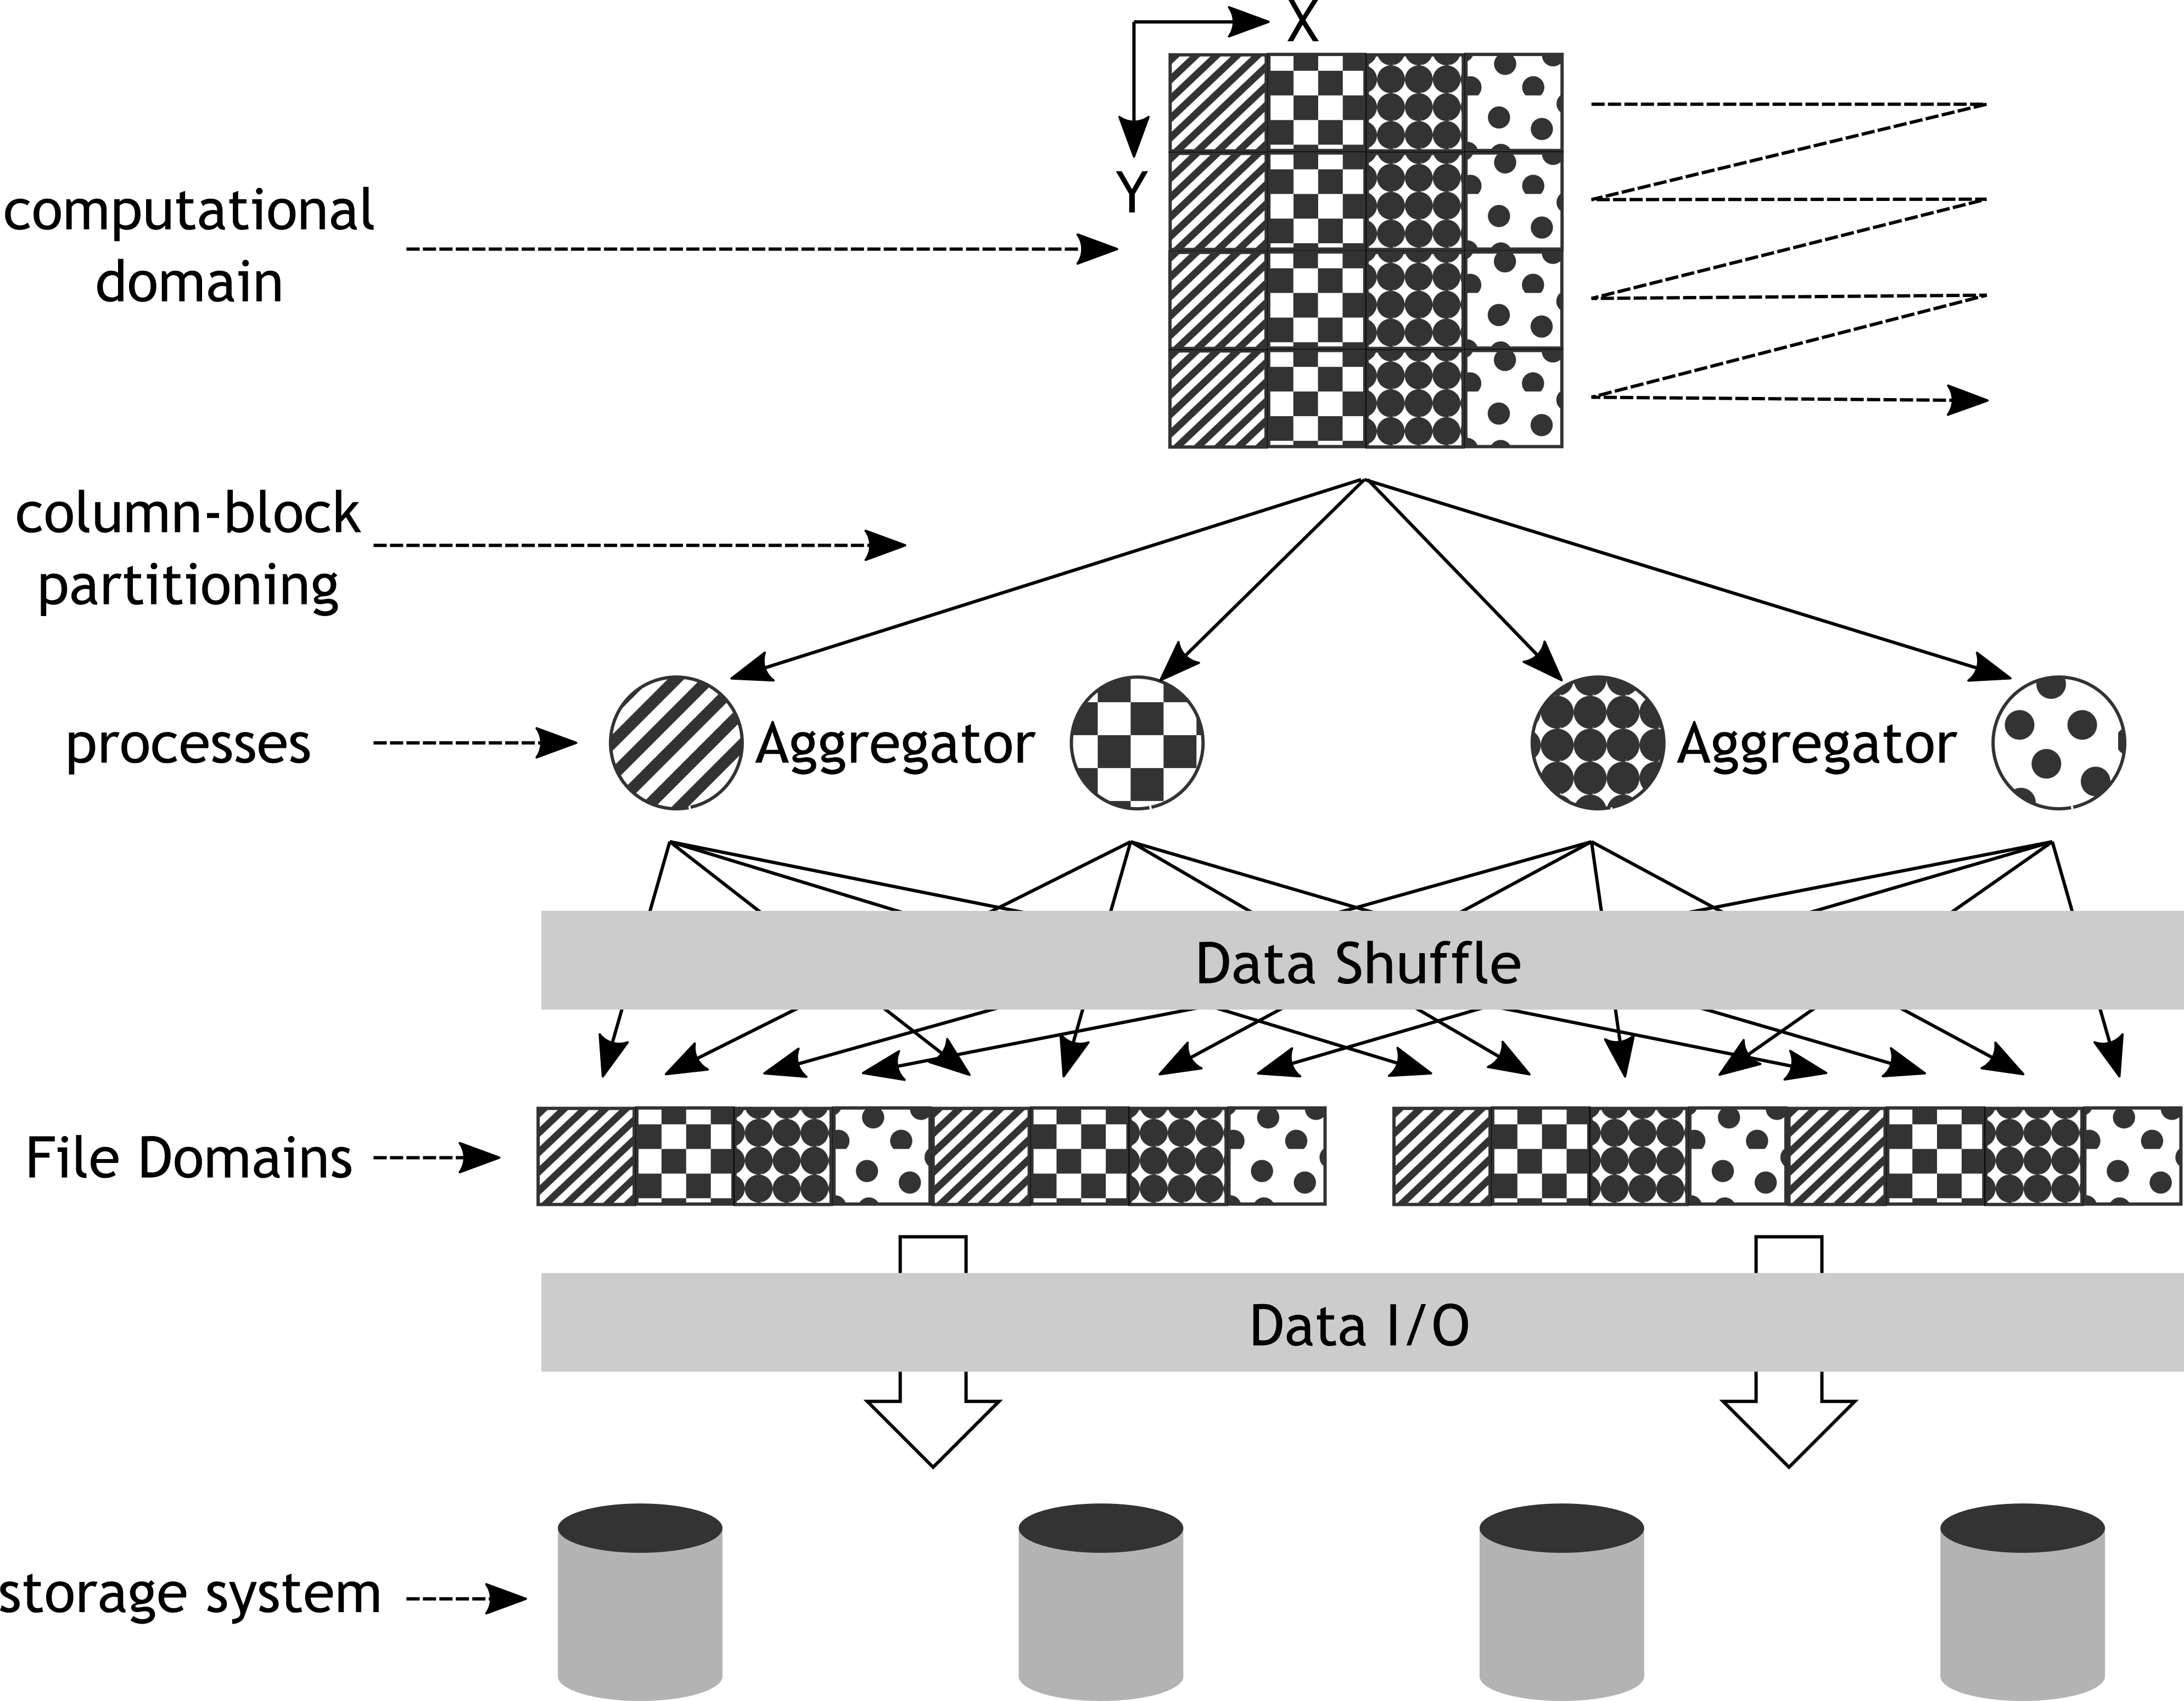
\includegraphics[width=0.8\textwidth]{figures/twophase}
  \caption{Simplified two phase I/O scheme. A two-dimensional domain is partitioned among four processes in the parallel application using a column-block strategy. Data is then rearranged to form an 
  intermediate pattern that matches the logical data organization in the file. This pattern is afterwards used by the two aggregators to access the storage system.}
  \label{figure: coll_io}
\end{figure}

%Even when processes generate large I/O requests, it might be still beneficial to coordinate them to reduce parallel file system block locking contention as well as concurrency level on data servers. 
This mechanism effectively adapts the I/O pattern to the characteristics of the file system, extracting maximum performance from it. Figure~\ref{figure: coll_io} exemplifies the basic two phase I/O 
mechanism just described. In the figure there are four processes, two of which play the role of aggregators. Two phase I/O proceeds in two stages: \textit{data shuffling} and \textit{data I/O}. Data 
shuffling takes place between all the processes and aggregators and is aimed to build the logically contiguous file regions, also called \textit{file domains}, that will be later accessed during the 
data I/O phase. In the example shown in Figure~\ref{figure: coll_io}, the ext2ph algorithm converts the original column-block partitioning generated by the application into a row-block partitioning that 
matches the row-major mapping of data in the file.

Summarizing, the ext2ph has the following benefits: \textbf{(a)} improves disk utilization by converting small non-contiguous requests into large sequential accesses; \textbf{(b)} reduces block 
contention, and thus lock manager overhead, in POSIX compliant file systems. (In fact even when processes generate large I/O requests, it might still be beneficial to coordinate them to reduce file system
block locking contention as well as concurrency level on I/O servers.) Additionally, ext2ph also: \textbf{(c)} improves network utilization by reducing the number of remote procedure calls sent to I/O 
servers by file system clients; and \textbf{(d)} reduces load imbalance on I/O servers.

\subsection{Parallel Log structured File System}
PLFS~\cite{Bent2009} is an I/O middleware developed at the Los Alamos National Laboratory. It converts N-1 checkpoint patterns into N-N checkpoint patterns, thus moving the burden from file system lock 
contention to metadata creation operations. As shown in Figure~\ref{figure: plfs}, PLFS works as translation layer between the application and the parallel file system, and can perform its manipulations
transparently to the application through a FUSE module that runs on every node. This allows PLFS to exploit the underlying parallel file system infrastructure for data distribution and protection 
across I/O servers and only focus on the layout manipulation of checkpoint data.

As the figure shows, a new container, represented by a directory in the physical file system, is created for every new checkpoint. The checkpoint container includes, among other things, logical
file metadata and access permissions. For every node, PLFS also creates a new subdirectory in the main container to accommodate one file per process. This allows the N-N transformation giving every
process an independent physical file to work with. For every node an index file is also stored, which contains mapping information to reconstruct the original file layout during read operations. 
Mapping data consists of offsets and lengths of each write call.

\begin{figure}
\centering
\includegraphics[width=0.8\textwidth]{figures/plfs}
\caption{Pictorial representation of the PLFS translation mechanism that converts original application N-1 patterns into N-N patterns.}
\label{figure: plfs}
\end{figure}

As already said, the N-N pattern strategy moves the performance bottleneck from the file system lock manager to the metadata servers, that in this case have to handle a possibly large number of concurrent file
create requests. Another problem with the N-N strategy used in PLFS is that reading back checkpoiting data involves the open of many index files (one per node), from each of the N processes. Indeed, the mapping 
data in these files needs to be aggregated in order to be able to reconstruct the original layout in the logical file. For these reasons, in PLFS, I/O time is dominated by metadata operations. This has led 
to improvements of the original PLFS version that address metadata performance issues in the underlying parallel file system. In particular, Manzanares et al.~\cite{Adam2011} have proposed different alternatives 
for reading the index data. All the solutions move the aggregation of information from the file system level to the network level using MPI. For example, instead of allowing every process to read every index file
independently, only one process can read all index files and afterwards distribute the mapping across the network, thus bypassing the file system. The same work addresses the problem of metadata server congestion 
during file creation by federating multiple metadata servers, handling different mount points in the file system (Panasas PanFS~\cite{Welch2004} was used in this case), and distributing nodes' subdirectories among 
them.

\subsection{Scalable Checkpoint Restart Library}
SCR~\cite{Moody2010_2}~\cite{Moody2010} is a library for multi-level checkpoint restart developed at Lawrence Livermore National Laboratory and targeting N-N checkpointing patterns. It derives from two key 
observations on applications running on HPC systems. The first observation is that jobs, only need the most recent checkpoint in order to restart. The second observation is that even in the case of failures, 
the number of affected nodes is typically limited to one or two. Therefore, HPC jobs can overbook the system to have an additional small number of spare nodes that can takeover the crashed ones when needed.
Because only a limited number of nodes fail, and because writing data to the parallel file system can be a very slow operation, SCR uses local storage resources in compute nodes to store data. These can be RAM 
disks, hard disks or solid state drives. Local checkpoint are flushed to the parallel file system infrequently, thus reducing performance degradation and overload of storage system components that are more 
prone to failure when heavily stressed.

SCR can replicate information on local nodes across the network using MPI. There are three different replication strategies supported: \textit{LOCAL}, \textit{PARTNER} and \textit{XOR}. The LOCAL strategy does not 
replicate data at all, only a local copy is kept; the PARTNER strategy replicates each file for every process into another partner node; finally, the XOR strategy uses XOR to write parity data across multiple nodes. 
The PARTNER replication can withstand the failure of only one node, while the XOR replication uses RAID-5 and can thus withstand the failure of multiple nodes as long as they do not belong to the same parity group. 
When an application fails because of a node crash, SCR tries to recover the data from the local storage. If it is successful it can either restart the application, if there are enough spare resources, or can flush 
all the local checkpoints to the parallel file system. In the latter case the job will be restarted at a later time by reading the checkpoints from the parallel file system.

\subsection{SIONlib}
SIONlib~\cite{Frings2009}~\cite{Freche2009} is an I/O middleware developed at the Juelich Supercomputing Center in Germany. It addresses the problem of metadata performance in N-N checkpointing patterns by converting 
these into N-M patterns, where M is a smaller number of larger files (also called multifiles), most commonly equal to 1. Like the previously described PLFS, SIONlib is positioned between the application and the parallel 
file system, but unlike PLFS it requires modification of the target application in order to perform its transformations. For this purpose it provides an I/O API similar to ANSI C that processes (or tasks) use to access 
their independent files (or task-local files).

\begin{figure}[!htb]
\centering
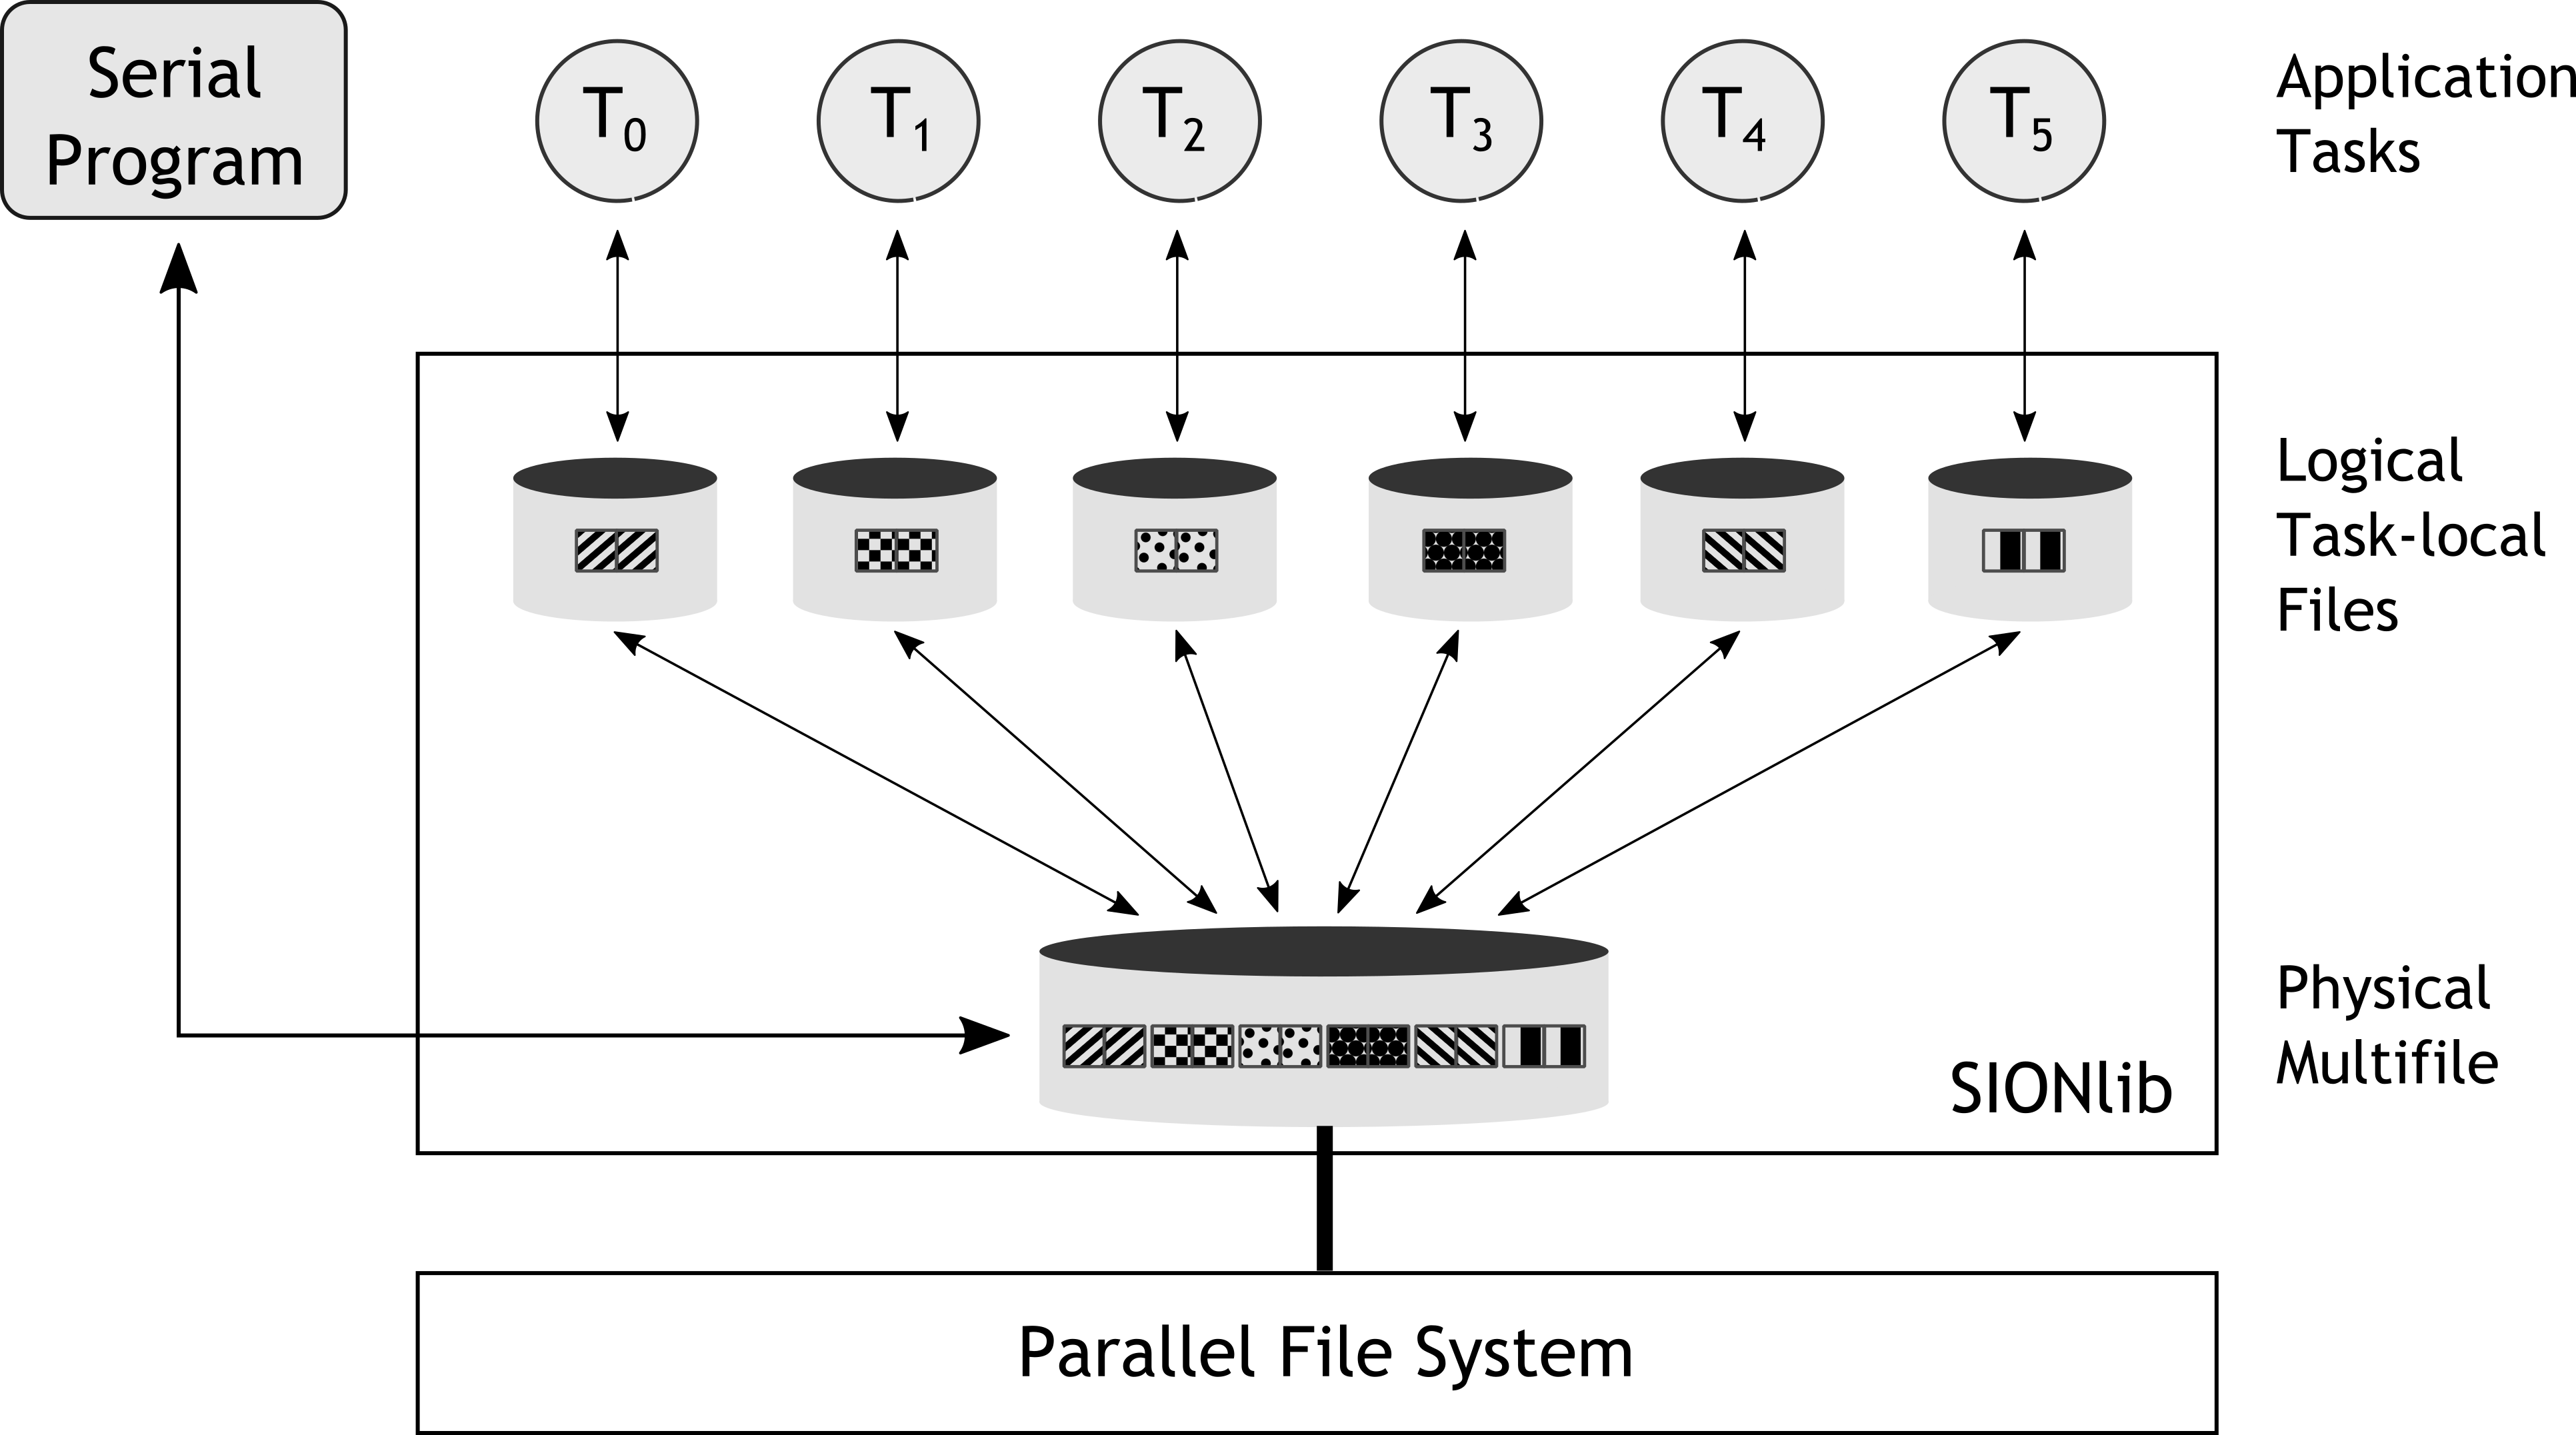
\includegraphics[width=\textwidth]{figures/sionlib}
\caption{Simplified representation of the SIONlib translation mechanism. A large number of task-local files is mapped into a smaller number of multifiles.}
\label{figure: sionlib}
\end{figure}

In SIONlib data from independent task-local files is not rearranged to reconstruct the layout that it would have had if it was written to a shared file directly; that is, SIONlib merely unifies the address space
of independent files into a larger address space without recreating a strided I/O pattern. Each task writes its data segments to the file independently, thus avoiding additional network communication overhead 
like in two phase I/O. To guarantee that data segments do not collide to the same stripe, these are naturally aligned to the file system boundaries. 

Since the amount of data written by every task may vary, SIONlib 
needs to allocate chunks of data in the multifile for each of them upfront; the size of the chunk is estimated by taking the largest write among all. Chunks are organized into adjacent blocks in the multifile, in this 
way if tasks exceed the chunk size they can write the additional data into a new chunk in the next block. Additional metadata is written at the beginning and at the end of the multifile to keep track of the data 
distribution into chunks and blocks. Because SIONlib does not rearrange file data in the multifiles but just groups independent files under a unique container, multifiles cannot be used to restart an application using 
a different task configuration. Indeed, in this case the amount of data would change with the number of processes, breaking the original layout.

Most recently, in the context of the DEEP-ER project\footnote{www.deep-er.eu}, SIONlib has been extended with multi-level checkpointing capabilities that allow applications to replicate checkpoints using a PARTNER 
configuration, like in the SCR library, also called \textit{buddy checkpoiting}. Additionally, the library supports a XOR checkpointing configuration through an additional memory component developed during the course 
of the project and called \textit{network attached memory} (NAM). When using the NAM, every task writes data to local storage and also sends a copy to the NAM, which computes and stores the parity information. If a node 
fails the NAM retrieves the survived nodes' data and reconstructs the failed node information through XOR with the parity previously stored.

\subsection{Adaptable I/O System}
ADIOS~\cite{Lofstead2008}~\cite{Liu2014} is an adaptable I/O middleware developed at the Oak Ridge National Laboratory. The key points on which ADIOS is built are: \textbf{(a)} the need for porting scientific codes 
from one system to another without changing I/O APIs. This also includes the possibility to add richer metadata annotations to the data, currently supported by other libraries like HDF5 and netCDF; \textbf{(b)} the 
need for supporting advanced technique for asynchronous I/O, thus allowing the application to be free to progress with computation while the middleware takes care of moving data to the file system; and finally, 
\textbf{(c)} the need for integrating scientific codes with additional tools for post processing and data visualization. In this sense, while previously reviewed middlewares focus on raw I/O performance, ADIOS provides 
an holistic approach to I/O that embraces all the aspects of data generation and exploitation.

ADIOS achieves the first goal by providing a simple flexible interface that applications can use to perform their I/O. Nevertheless, the actual I/O transport method is not determined at the application level but instead 
configured using an external XML file. This effectively makes applications portable from one system to another and allows flexible data representations that can include richer metadata annotations. 
Moreover, public I/O methods can be overloaded to send trigger messages to other tools (e.g., visualization tools) that can thus be notified when new data becomes available for processing. Like previously reviewed middlewares, 
ADIOS supports N-N, N-M and N-1 patterns. When using N-1 and N-M patterns, ADIOS avoids data reorganization, and thus global synchronization, by allowing every process to write independently to the file; like in SIONlib, 
this is possible through a custom binary format (BP-ADIOS).
